% !TeX program = pdflatex
\documentclass[11pt]{article}

\usepackage[margin=1in]{geometry}
\usepackage{lmodern}
\usepackage{microtype}
\usepackage{setspace}
\onehalfspacing

\usepackage{amsmath,amssymb,amsfonts,mathtools,bm,booktabs,tabularx,array}
\usepackage{graphicx}
\usepackage{xcolor}
\usepackage{tikz}
\usetikzlibrary{arrows.meta,calc,fit,positioning}
\usepackage{enumitem}
\usepackage[round,authoryear]{natbib}
\usepackage{hyperref}
\hypersetup{colorlinks=true,linkcolor=black,citecolor=black,urlcolor=black}

\newcommand{\R}{\mathbb{R}}
\newcommand{\Rp}{\mathbb{R}_{+}}
\newcommand{\E}{\mathbb{E}}
\newcommand{\Var}{\operatorname{Var}}
\newcommand{\tr}{\operatorname{tr}}
\newcommand{\diag}{\operatorname{diag}}
\newcommand{\vect}[1]{\bm{#1}}
\newcommand{\mat}[1]{\bm{#1}}
\newcommand{\Id}[1]{\mat I_{#1}}
\newcommand{\zeros}[1]{\vect 0_{#1}}
\newcommand{\ones}[1]{\vect 1_{#1}}
\newcommand{\ind}{\mathbf{1}}
\newcommand{\Normal}{\mathcal{N}}
\newcommand{\TN}{\mathcal{N}^{+}}
\newcommand{\IG}{\operatorname{IG}}
\newcommand{\GIG}{\operatorname{GIG}}
\newcommand{\Exp}{\operatorname{Exp}}
\newcommand{\Unif}{\operatorname{Unif}}
\newcommand{\AL}{\operatorname{AL}}
\newcommand{\exAL}{\operatorname{exAL}}
\newcommand{\RHS}{\ensuremath{\operatorname{RHS}}}
\newcommand{\aCRPS}{\operatorname{aCRPS}}
\newcommand{\elbo}{\mathcal{L}}
\newcommand{\logit}{\operatorname{logit}}
\newcommand{\expit}{\operatorname{expit}}
\DeclareMathOperator{\argmin}{arg\,min}
\newcommand{\pkg}[1]{\textsf{#1}}
\newcommand{\figalt}[1]{}
\newcommand{\TableStyle}{\footnotesize\setlength{\tabcolsep}{4pt}\renewcommand{\arraystretch}{1.08}}

% Article-facing current-output aliases for the GloFAS application section.
\newcommand{\GlofasApplicationCurrentScoreTable}{tables/glofas_application_current_score_summary.tex}
\newcommand{\GlofasApplicationCurrentCorrectedPathsFigure}{figures/glofas_application/glofas_qdesn_discrepancy_corrected_quantile_paths__glofas_stage_n_winner_scorebalanced_20260703.pdf}
\newcommand{\GlofasApplicationCurrentForecastWindowFigure}{figures/glofas_application/diagnostics/glofas_stage_n_winner_full7_scorebalanced_qdesn_synthesized_bands__glofas_stage_n_winner_scorebalanced_20260703.pdf}
\newcommand{\GlofasApplicationCurrentQdesnCheckLoss}{0.3339}
\newcommand{\GlofasApplicationCurrentRawCheckLoss}{0.7639}
\newcommand{\GlofasApplicationCurrentCheckLossReduction}{56.3\%}
\newcommand{\GlofasApplicationCurrentQdesnIntervalScore}{4.1402}
\newcommand{\GlofasApplicationCurrentRawIntervalScore}{13.0538}
\newcommand{\GlofasApplicationCurrentIntervalScoreReduction}{68.3\%}
\newcommand{\GlofasApplicationCurrentQdesnCrps}{0.6859}
\newcommand{\GlofasApplicationCurrentRawCrps}{1.4424}
\newcommand{\GlofasApplicationCurrentCrpsReduction}{52.4\%}
\newcommand{\GlofasApplicationCurrentQdesnMeanCoverage}{0.833}
\newcommand{\GlofasApplicationCurrentRawMeanCoverage}{0.000}
\newcommand{\GlofasApplicationCurrentScoredHorizons}{28}
\newcommand{\GlofasApplicationCurrentOriginDate}{2022-12-25}
\newcommand{\GlofasApplicationCurrentVbIterations}{median 150; max 150}
\newcommand{\GlofasApplicationCurrentReferenceReservoirDepth}{4}
\newcommand{\GlofasApplicationCurrentReferenceReservoirSize}{100,100,100,100}
\newcommand{\GlofasApplicationCurrentReferenceReducerSize}{100,100,100}
\newcommand{\GlofasApplicationCurrentReferenceReservoirMemory}{300}
\newcommand{\GlofasApplicationCurrentReferenceReservoirWashout}{500}
\newcommand{\GlofasApplicationCurrentReferenceReservoirAlpha}{0.0225,0.0225,0.0225,0.0225}
\newcommand{\GlofasApplicationCurrentReferenceReservoirRho}{0.95,0.95,0.95,0.95}
\newcommand{\GlofasApplicationCurrentReferenceReservoirPiW}{0.03,0.03,0.03,0.03}
\newcommand{\GlofasApplicationCurrentReferenceReservoirPiIn}{1,1,1,1}
\newcommand{\GlofasApplicationCurrentReferenceReservoirWinScaleGlobal}{0.16}
\newcommand{\GlofasApplicationCurrentReferenceReservoirWinScaleBias}{0.16}
\newcommand{\GlofasApplicationCurrentReferenceReservoirSeed}{20260512}
\newcommand{\GlofasApplicationCurrentDiscrepancyReservoirDepth}{4}
\newcommand{\GlofasApplicationCurrentDiscrepancyReservoirSize}{100,100,100,100}
\newcommand{\GlofasApplicationCurrentDiscrepancyReducerSize}{100,100,100}
\newcommand{\GlofasApplicationCurrentDiscrepancyReservoirMemory}{300}
\newcommand{\GlofasApplicationCurrentDiscrepancyReservoirWashout}{500}
\newcommand{\GlofasApplicationCurrentDiscrepancyReservoirAlpha}{0.0075,0.0075,0.0075,0.0075}
\newcommand{\GlofasApplicationCurrentDiscrepancyReservoirRho}{0.95,0.95,0.95,0.95}
\newcommand{\GlofasApplicationCurrentDiscrepancyReservoirPiW}{0.03,0.03,0.03,0.03}
\newcommand{\GlofasApplicationCurrentDiscrepancyReservoirPiIn}{1,1,1,1}
\newcommand{\GlofasApplicationCurrentDiscrepancyReservoirWinScaleGlobal}{0.28}
\newcommand{\GlofasApplicationCurrentDiscrepancyReservoirWinScaleBias}{0.28}
\newcommand{\GlofasApplicationCurrentDiscrepancyReservoirSeed}{20261521}
\newcommand{\GlofasApplicationCurrentSharedRhsTau}{0.001}
\newcommand{\GlofasApplicationCurrentDiscrepancyRhsTau}{0.03}
\newcommand{\GlofasApplicationCurrentSpreadCalibrationFactor}{1.4}
\newcommand{\GlofasApplicationCurrentSpreadCalibrationAdditiveWidth}{0.5}
\newcommand{\GlofasApplicationCurrentSpreadCalibrationCenterQuantile}{0.50}

% Reported current-output aliases for the full PriceFM benchmark section.
\newcommand{\PricefmFullRegionFolds}{114}
\newcommand{\PricefmFullRegions}{38}
\newcommand{\PricefmFullFolds}{3}
\newcommand{\PricefmFullQdesnWins}{66}
\newcommand{\PricefmFullQdesnClose}{12}
\newcommand{\PricefmFullPricefmWins}{36}
\newcommand{\PricefmFullQdesnWinRate}{57.9\%}
\newcommand{\PricefmFullMeanQdesnAql}{6.826}
\newcommand{\PricefmFullMeanPricefmAql}{7.039}
\newcommand{\PricefmFullMeanDeltaAql}{-0.213}
\newcommand{\PricefmFullMedianDeltaAql}{-0.083}
\newcommand{\PricefmFullGraphRows}{56}
\newcommand{\PricefmFullTargetOnlyRows}{58}
\newcommand{\PricefmFullHorizonRows}{72}
\newcommand{\PricefmFullPaperQuantiles}{0.10, 0.25, 0.45, 0.50, 0.55, 0.75, 0.90}
\newcommand{\PricefmFullMainSummaryTable}{tables/pricefm_full_main_summary.tex}

\input{figures/quantile_initialization/quantile_initialization_styles.tex}

\newcounter{suppalgorithm}
\renewcommand{\thesuppalgorithm}{S\arabic{suppalgorithm}}
\newenvironment{suppalgorithm}[1]{%
  \refstepcounter{suppalgorithm}%
  \par\medskip\noindent\textbf{Algorithm~\thesuppalgorithm. #1.}\par
  \nopagebreak[4]\smallskip\nopagebreak[4]
}{\par\medskip}

\renewcommand{\theequation}{S\arabic{equation}}
\renewcommand{\thetable}{S\arabic{table}}
\renewcommand{\thesection}{S\arabic{section}}
\renewcommand{\thesubsection}{S\arabic{section}.\arabic{subsection}}
\renewcommand{\thesubsubsection}{S\arabic{section}.\arabic{subsection}.\arabic{subsubsection}}

\title{Supplementary Material for ``Bayesian Quantile Deep Echo State Networks for Nonlinear Time Series''}
\author{Antonio De Leon \and Raquel Prado \and Bruno Sans\'o}
\date{August 28, 2026}

\begin{document}
\maketitle

\begin{abstract}
\noindent
Conditional on the fixed nonlinear features generated by a deep echo state
network (DESN), the quantile deep echo state network (Q--DESN) is a
high-dimensional Bayesian quantile regression model. We use the asymmetric
Laplace (AL) working likelihood and, under the label exAL, the quantile-fixed
generalized asymmetric Laplace distribution of \citet{yan2025new}. The
posterior includes regression coefficients, likelihood scale and asymmetry
parameters, auxiliary mixture variables, and shrinkage parameters. This
supplement derives the augmented posterior under Gaussian ridge and
Nishimura--Suchard regularized-horseshoe priors, the full conditional
distributions for Markov chain Monte Carlo (MCMC), and the coordinate updates
and evidence lower bound for variational Bayes with the Laplace--Delta
approximation (VB--LD). It also develops the joint multi-quantile regression
with regularized-horseshoe shrinkage on adjacent coefficient differences and
provides additional simulation and application results.
\end{abstract}

\section{Purpose and Relation to the Main Article}
\label{sec:supp_relation_main}

The main article introduces Q--DESN, defines its fixed deep reservoir feature
map, and presents the simulation design. Once
the reservoir weights, input weights, reducers, leak rates, and washout
convention are fixed, the likelihood depends on the data only through a
deterministic design matrix
\(\mat X=[\vect x_1^\top;\ldots;\vect x_T^\top]\). Thus the
Q--DESN regression is a static Bayesian quantile regression problem with a
high-dimensional nonlinear design. Consequently, the static AL and exAL
regression derivations used by \pkg{exdqlm}
\citep{barata2021_flex_quantile,exdqlmRPackage} can be adapted to the
Q--DESN regression by replacing ordinary covariate rows with rows of the fixed
DESN design matrix.

This supplement derives the augmented posterior, full conditional
distributions, mean-field coordinate updates, and evidence lower bound. Gaussian
ridge is the baseline coefficient prior, and RHS denotes the regularized
horseshoe. The software label \texttt{rhs\_ns} identifies the
Nishimura--Suchard product representation used to obtain closed-form scale
updates. For exAL, Taylor and Laplace approximations are evaluated separately
for \(\gamma<0\) and \(\gamma>0\); the point \(\gamma=0\) is handled under the
nested AL model. Subsequent sections cover reservoir specification, the
fixed-design likelihood and prior, MCMC and variational computation, the joint
quantile-vector extension, monotone rearrangement, supplementary empirical
results, and the GloFAS latent-path ensemble-likelihood model.

\section{Reservoir Specification, Selection, and Diagnostics}
\label{sec:supp_reservoir_diagnostics}

Table~\ref{tab:supp-reservoir-selection} summarizes the reservoir-design
quantities and their associated diagnostics. Posterior inference conditions on
the resulting feature map and quantifies uncertainty in the regression,
likelihood, and shrinkage parameters.

\begin{table}[!htbp]
\centering
\begingroup
\TableStyle
\begin{tabularx}{\textwidth}{@{}>{\raggedright\arraybackslash}p{0.16\textwidth}
>{\raggedright\arraybackslash}p{0.25\textwidth}
>{\raggedright\arraybackslash}p{0.28\textwidth}
>{\raggedright\arraybackslash}X@{}}
\toprule
Component & Role in the fixed feature map & Design consideration & Potential concern \\
\midrule
\(D\) & Number of reservoir layers and hierarchy of time scales &
Evaluate a small prespecified set and retain additional depth only when
validation forecast criteria improve consistently across reservoir realizations. &
Unnecessary depth can add numerically unstable or redundant design columns. \\
\(\{n_d\},\{\tilde n_d\}\) & Number of reservoir states and lower-layer feature
dimension & Treat as the main complexity control, with reduction sizes chosen
as part of the same feature map. &
A large design relative to the sample size can yield weakly identified
coefficients or a poorly conditioned regression; redundant states can reduce
the effective rank of \(\mat X\). \\
\(m\) & Explicit lag memory entering the reservoir input & Choose a
domain-informed grid and require all lags to be available at the forecast
origin. & Excessive lags increase dimension and can incorporate observations
unavailable at the forecast origin if alignment is incorrect. \\
\(\{\alpha_d\},\{\rho_d\}\) & Reservoir time scale, persistence, and stability &
Compare jointly because both affect memory. Near-one radii require empirical
stability checks. & States concentrated near the activation bounds,
near-constant states, or sensitivity to initial conditions. \\
\(\{\pi^{(W)}_d\},\{\pi^{(\mathrm{in})}_d\}\) and input scaling & Recurrent
connectivity and input-induced variation & Fix from a small set of literature-guided
defaults; broaden the comparison when diagnostics show weak state variation or
concentration near the activation bounds. & Low connectivity can produce weakly
varying states; high connectivity or input scaling can concentrate states near
the activation bounds. \\
\(f,k,T_0\) & Nonlinearity, transformation of reduced lower-layer states, and initial-condition
washout & Fix before feature-map comparison, with \(T_0\) chosen relative to the
memory scale. & Short washout can leave initial-condition artifacts. \\
Random reservoir realization & Realization of the random feature map & Assess
variation across repeated reservoir realizations. &
Held-out scores can vary materially across realizations. \\
\bottomrule
\end{tabularx}
\endgroup
\caption{Reservoir specification and diagnostics for the fixed
Q--DESN feature map.}
\label{tab:supp-reservoir-selection}
\end{table}

\subsection{Validation-Based Selection and Initialization}
\label{sec:supp_selection_initialization}

For a fixed statistical specification \(M\), reservoir candidates
\(R_j\) are compared on the designated validation observations using
the criterion stated for the analysis. The response convention, information
set, design rows, transformations, feature ordering, scaling quantities, and
forecast definition are held common across candidates. Reservoir states are
also checked for finite values, concentration near the activation bounds,
near-constant columns, and severe numerical dependence. The selected
specification satisfies
\[
\widehat R_M
\in
\argmin_{R_j:\,j=1,\ldots,J}
S_{\mathrm{val}}(R_j;M).
\]
The selected \(\widehat R_M\) is held fixed for
evaluation.

Suppose that the probability grid satisfies
\(p_1<\cdots<p_m=0.50<\cdots<p_K\).
After the Gaussian ridge and Gaussian \(\RHS\)--VB fits, compatible estimates
from the latter initialize the median AL regression. The lower side of the AL
grid is fitted in the order
\[
0.50\ \longrightarrow\ p_{m-1}\ \longrightarrow\ \cdots\
\longrightarrow\ p_1,
\]
and the upper side is fitted in the order
\[
0.50\ \longrightarrow\ p_{m+1}\ \longrightarrow\ \cdots\
\longrightarrow\ p_K.
\]
Thus each AL regression is initialized from the nearest completed level on the
same side of the median. For every \(k=1,\ldots,K\), the completed AL fit at
\(p_k\) initializes the exAL fit at \(p_k\). The exAL regressions may
therefore be fitted as soon as their matching AL fits are available.

The joint AL regression is initialized from the complete collection of
independent AL fits, and the joint exAL regression is initialized from the
complete collection of independent exAL fits. Let
\(\widehat\beta_{0k}^{\,\mathrm{ind}}\) and
\(\widehat{\vect\beta}_k^{\,\mathrm{ind}}\) denote the independent
intercept and slope estimates from the matching likelihood family. Initial
values for the level-specific joint coefficients are
\[
\beta_{0k}^{(0)}
=\widehat\beta_{0k}^{\,\mathrm{ind}},
\qquad
\vect\beta_k^{(0)}
=\widehat{\vect\beta}_k^{\,\mathrm{ind}},
\qquad k=1,\ldots,K.
\]
Under the adjacent-difference parameterization in
Section~\ref{sec:joint_qdesn_supp}, the corresponding initial differences are
\begin{equation}
\vect\Delta_k^{(0)}
=\widehat{\vect\beta}_k^{\,\mathrm{ind}}
-\widehat{\vect\beta}_{k-1}^{\,\mathrm{ind}},
\qquad k=2,\ldots,K.
\label{eq:supp-joint-initial-differences}
\end{equation}
Independent AL estimates are used for joint AL, and independent exAL estimates
are used for joint exAL in Eq.~\eqref{eq:supp-joint-initial-differences}.

When the source and destination models differ, only parameters with
corresponding interpretations are used to construct starting values. Gaussian
residual scale and AL or exAL scale have different parameterizations, so the
initial value of the destination scale is obtained under its own
parameterization. Parameters specific to the exAL likelihood or coefficient
prior are initialized within their respective supports. For a VB-to-MCMC
initialization, the response, data period, design matrix, feature ordering,
transformations, reservoir realization, likelihood, probability level or grid,
parameterization, and prior specification agree. MCMC then targets the
posterior distribution of that same model. Convergence is assessed using the
diagnostics stated for the empirical analysis.

\begin{figure}[!htbp]
  \centering
  \input{figures/quantile_initialization/quantile_initialization_picture.tex}
  \caption[Sequential initialization centered at the median]{%
    \input{figures/quantile_initialization/quantile_initialization_caption.tex}%
  }
  \figalt{A Gaussian ridge regression initializes a Gaussian regularized-horseshoe
  variational fit, which initializes the median AL regression. Independent AL
  fits then proceed outward toward both tails; each initializes the exAL fit at
  the same probability level. Complete independent grids initialize the
  corresponding joint models, and fitted variational models initialize MCMC.}
  \label{fig:supp-quantile-sequential-initialization}
\end{figure}

\section{Distributional Conventions}
\label{sec:dist_conventions}

\noindent\textbf{Shared parameterizations.}
The posterior kernels below use the following distributional
parameterizations. These conventions are used in the MCMC,
coordinate-ascent variational inference (CAVI), and evidence lower bound (ELBO)
derivations below; in particular, all inverse-gamma distributions use a rate in
the reciprocal scale.

The inverse-gamma (IG) parameterization is
\[
p(x\mid a,b)=\frac{b^a}{\Gamma(a)}x^{-a-1}\exp(-b/x),\qquad x>0,
\]
and the generalized inverse Gaussian (GIG) parameterization
\[
p(x\mid \lambda,\chi,\psi)
\propto x^{\lambda-1}\exp\left\{-\frac12(\chi/x+\psi x)\right\},
\qquad x>0.
\]
The notation \(\TN(m,V)\) denotes a Normal distribution with mean \(m\) and
variance \(V\), truncated to \((0,\infty)\). The functions \(\Phi\) and
\(\phi\) denote the standard Normal distribution and density functions.

\noindent\textbf{AL constants.}
For a fixed target quantile \(p_0\in(0,1)\), the AL constants are
\[
A_0=\frac{1-2p_0}{p_0(1-p_0)},\qquad
B_0=\frac{2}{p_0(1-p_0)}.
\]
\noindent\textbf{exAL branch constants.}
The notation \(\exAL\) denotes the quantile-fixed generalized asymmetric
Laplace distribution of \citet{yan2025new}. This convention emphasizes the
role of the likelihood as an extension of AL while preserving the
quantile-fixed parameterization that identifies \(\mu\) as the target
conditional quantile. The exAL likelihood
introduces an asymmetry parameter \(\gamma\in(L,U)\), where \(L\) and
\(U\) are determined by the quantile-identifying construction. Define
\[
g(\gamma)=2\Phi(-|\gamma|)\exp(\gamma^2/2),\qquad
p_\gamma=\ind\{\gamma<0\}
+\frac{p_0-\ind\{\gamma<0\}}{g(\gamma)}.
\]
Then, with the fixed probability level shown explicitly when needed,
\[
\begin{alignedat}{2}
A_{p_0}(\gamma)\equiv A_\gamma
&=\frac{1-2p_\gamma}{p_\gamma(1-p_\gamma)},
&\qquad B_{p_0}(\gamma)\equiv B_\gamma
&=\frac{2}{p_\gamma(1-p_\gamma)},\\
C_\gamma&=\{\ind\{\gamma>0\}-p_\gamma\}^{-1},
& D_\gamma\equiv D_{p_0}(\gamma)&=C_\gamma|\gamma|.
\end{alignedat}
\]
The shorthand \(D_\gamma\) reduces visual clutter in posterior kernels and is
distinct from the regularized-horseshoe local scales \(\lambda_j\).

\noindent\textbf{AL nesting and branchwise regularity.}
When \(\gamma=0\) and the \(s_t\) latents are omitted, the exAL hierarchy
reduces to the AL working likelihood with constants \(A_0,B_0\).
This nesting is exact. The surrounding \(p_\gamma\), \(A_\gamma\),
\(B_\gamma\), and \(D_\gamma\) maps are branchwise smooth for
\(\gamma<0\) and \(\gamma>0\), but the absolute value and indicator branches
make generic two-sided derivative statements at \(\gamma=0\) invalid except in
special symmetric cases. In particular, the one-sided derivatives of
\(p_\gamma\) at zero are proportional to \(1-p_0\) from the left and to
\(p_0\) from the right. At \(\gamma=0\), calculations use the nested AL model;
for \(\gamma\ne0\), numerical derivatives are evaluated within the
corresponding sign region.

\section{DESN Feature Map and Fixed-Design Quantile Regression}
\label{sec:desn_features}

The Q--DESN regression inherits the feature map defined in the main article. The
reservoir weights, input weights, reducers, leak rates, and washout convention
are fixed before posterior inference. Posterior inference conditions on the
design matrix \(\mat X\) constructed from these features. Scalar responses are denoted by
lowercase \(y_t\), both in likelihood statements and posterior kernels.

Let \(\vect u_t=(y_{t-1},\ldots,y_{t-m},\vect z_t^\top)^\top\) collect response
lags and exogenous covariates. For layers \(d=1,\ldots,D\), Q--DESN draws sparse
reservoir matrices \(\mat W_d\), input matrices \(\mat W^{\mathrm{in}}_d\), and
optional reducers \(\mat Q_d\), \(d=1,\ldots,D-1\), once and keeps them fixed.
With layer-specific leak rates \(\alpha_d\), activation \(f\), and spectral
radius targets \(\rho_d\),
the layer states satisfy
\begin{align}
\vect h_{t,1}
&=(1-\alpha_1)\vect h_{t-1,1}
+\alpha_1 f\{\bar{\mat W}_1\vect h_{t-1,1}+\mat W^{\mathrm{in}}_1\vect u_t\},
\label{eq:supp_desn_layer1}\\
\vect h_{t,d}
&=(1-\alpha_d)\vect h_{t-1,d}
+\alpha_d f\{\bar{\mat W}_d\vect h_{t-1,d}
+\mat W^{\mathrm{in}}_d\tilde{\vect h}_{t,d-1}\},\qquad d\ge2,
\label{eq:supp_desn_layerd}\\
\tilde{\vect h}_{t,d-1}&=\mat Q_{d-1}\vect h_{t,d-1},
\end{align}
where \(\bar{\mat W}_d=\rho_d\mat W_d/\rho(\mat W_d)\). The layer
recursions in Eqs.~\eqref{eq:supp_desn_layer1} and
\eqref{eq:supp_desn_layerd} define the fixed feature vector
\begin{equation}
\tilde{\vect x}_t
=\{ \vect h_{t,D}^\top,\ k(\tilde{\vect h}_{t,1})^\top,\ldots,
k(\tilde{\vect h}_{t,D-1})^\top,\ \vect u_t^\top\}^\top,
\qquad
\vect x_t=(1,\tilde{\vect x}_t^\top)^\top.
\label{eq:supp_feature_stack}
\end{equation}
After a fixed washout period, the reservoir quantities in
\eqref{eq:supp_feature_stack} are treated as deterministic. Let
\(\vect\beta=(\beta_0,\beta_1,\ldots,\beta_r)^\top\) and
\[
\mat X=[\vect x_1^\top;\ldots;\vect x_T^\top]\in\R^{T\times(r+1)},\qquad
\mu_t=\vect x_t^\top\vect\beta .
\]
All posterior inference is conditional on \(\mat X\).

\section{Q--DESN Working Likelihoods, Priors, and Augmented Posterior}
\label{sec:model_joint}

The augmented posterior densities below are used by both computational
schemes. The AL and exAL likelihoods are working likelihoods for a
fixed target quantile, while the auxiliary variables provide equivalent
mixture representations for computation.

\subsection{AL and exAL Augmented Likelihoods}

The exAL Q--DESN observation hierarchy is
\begin{align}
v_t\mid\sigma &\sim \Exp(\text{rate}=1/\sigma),&
s_t&\sim\TN(0,1),\\
y_t\mid\vect\beta,\sigma,\gamma,v_t,s_t,\mat X
&\sim
\Normal\left(
\vect x_t^\top\vect\beta+\sigma D_\gamma s_t+A_\gamma v_t,
\sigma B_\gamma v_t
\right).
\label{eq:supp_exal_hierarchy}
\end{align}
The marginal \(p_0\)-quantile of \(y_t\mid\vect x_t\) is
\(\vect x_t^\top\vect\beta\). The AL special case is
\begin{align}
v_t\mid\sigma &\sim \Exp(\text{rate}=1/\sigma),\\
y_t\mid\vect\beta,\sigma,v_t,\mat X
&\sim
\Normal\left(
\vect x_t^\top\vect\beta+A_0v_t,
\sigma B_0v_t
\right).
\label{eq:supp_al_hierarchy}
\end{align}

\subsection{Coefficient Priors}
\label{sec:priors}

The coefficient prior regularizes the high-dimensional regression after the
reservoir features have been fixed. The ridge prior is the default Gaussian
baseline. The regularized-horseshoe prior is the adaptive global-local shrinkage
alternative; its product representation keeps the local, global, and slab scale
updates in closed form.

For the ridge coefficient prior, let
\begin{equation}
\vect\beta\sim\Normal(\vect b_\beta,\mat V_\beta),
\qquad
\mat P_\beta=\mat V_\beta^{-1}.
\label{eq:supp_ridge_prior}
\end{equation}
Applications usually keep the intercept weakly regularized and use a
diagonal slope penalty, while \eqref{eq:supp_ridge_prior} allows a general
positive definite prior covariance.

For the regularized-horseshoe prior, the intercept is independent,
\(\beta_0\sim\Normal(b_0,V_0)\), and the non-intercept coefficients are
represented through the
Nishimura--Suchard-style regularized horseshoe construction
\citep{CarvalhoPolsonScott2010HS,PiironenVehtari2017RHS,NishimuraSuchard2023SSS}.
For \(j=1,\ldots,r\),
\begin{equation}
p_{\mathrm{ns}}(\beta_j,\lambda_j\mid\tau,\zeta)
\propto
\exp\left(-\frac{\beta_j^2}{2\tau^2\lambda_j^2}\right)
\exp\left(-\frac{\beta_j^2}{2\zeta^2}\right)
\lambda_j^{-1}(1+\lambda_j^2)^{-1}.
\label{eq:supp_ns_joint}
\end{equation}
Equation~\eqref{eq:supp_ns_joint} is the marginal joint description after the
half-Cauchy auxiliary variable for the local scale has been integrated out. The
MCMC and VB derivations use the corresponding augmented product
\[
\Normal(\beta_j\mid0,\tau^2\lambda_j^2)\,
\Normal(0\mid\beta_j,\zeta^2)
\]
together with inverse-gamma auxiliaries for \(\lambda_j^2\), \(\nu_j\),
\(\tau^2\), and \(\xi\). Normalizing factors that depend on the scale
parameters are retained. This augmented product representation is the one used
in the posterior densities below.
Equivalently, the conditional coefficient law is Gaussian with effective
variance
\begin{equation}
\beta_j\mid\lambda_j,\tau,\zeta
\sim
\Normal(0,V_j),\qquad
V_j=\left(\zeta^{-2}+\tau^{-2}\lambda_j^{-2}\right)^{-1}
=\frac{\zeta^2\tau^2\lambda_j^2}{\zeta^2+\tau^2\lambda_j^2}.
\label{eq:supp_rhs_cond_beta}
\end{equation}
Equation~\eqref{eq:supp_rhs_cond_beta} makes the finite-slab bound explicit.
For inverse-gamma scale updates, use the half-Cauchy augmentation
\citep{MakalicSchmidt2016SimpleSampler}:
\begin{align}
\lambda_j^2\mid\nu_j&\sim\IG(1/2,1/\nu_j),&
\nu_j&\sim\IG(1/2,1),\\
\tau^2\mid\xi&\sim\IG(1/2,1/\xi),&
\xi&\sim\IG(1/2,1/\tau_0^2),
\label{eq:supp_hs_aux}\\
\zeta^2&\sim\IG(a_\zeta,b_\zeta),
\label{eq:supp_zeta_prior}
\end{align}
The slab update in Eq.~\eqref{eq:supp_zeta_prior} is omitted when
\(\zeta^2\) is fixed.

\subsection{Reference Calibration of the Global Shrinkage Scale}
\label{subsec:supp-rhs-global-scale}

The hierarchy in Eq.~\eqref{eq:supp_hs_aux} distinguishes the posterior random
global scale \(\tau\) from the fixed hyperprior scale \(\tau_0\). The latter
should reflect the response scale, the amount of information in the fitting
sample, the number of penalized coefficients, and prior information about
coefficient activity. We first state the Gaussian reference calculation of
\citet{PiironenVehtari2017RHS} and then describe its use for Q--DESN.

Let \(N_{\mathrm{fit}}\) be the number of fitting observations, let \(r\) be
the number of standardized non-intercept columns, and let
\(\sigma_{\mathrm{ref}}>0\) be a residual-scale reference. Under an orthogonal
Gaussian design, the ordinary-horseshoe shrinkage factor for coefficient \(j\)
is
\begin{equation}
\kappa_j
=\left(1+
\frac{N_{\mathrm{fit}}\tau^2\lambda_j^2}
{\sigma_{\mathrm{ref}}^2}
\right)^{-1}.
\label{eq:supp-rhs-kappa-reference}
\end{equation}
If
\(m_{\mathrm{eff}}=\sum_{j=1}^r(1-\kappa_j)\), integration over the
half-Cauchy local scales gives
\begin{equation}
\E(m_{\mathrm{eff}}\mid\tau,\sigma_{\mathrm{ref}})
=r\frac{a}{1+a},
\qquad
a=\frac{\tau\sqrt{N_{\mathrm{fit}}}}{\sigma_{\mathrm{ref}}}.
\label{eq:supp-rhs-effective-size-reference}
\end{equation}
Equating Eq.~\eqref{eq:supp-rhs-effective-size-reference} to an elicited prior
reference \(m_0\in(0,r)\) and using the resulting scale for the half-Cauchy
hyperprior gives
\begin{equation}
\tau_{0,\mathrm{ref}}
=\frac{m_0}{r-m_0}
 \frac{\sigma_{\mathrm{ref}}}{\sqrt{N_{\mathrm{fit}}}}.
\label{eq:supp-rhs-tau0-gaussian-reference}
\end{equation}
Here \(m_0\) represents prior information about the number of coefficients
expected to escape strong global shrinkage; it is not a model size selected by
validation. When both the response and the penalized columns are standardized
using the fitting observations, setting \(\sigma_{\mathrm{ref}}=1\) gives the
unit-scale version of Eq.~\eqref{eq:supp-rhs-tau0-gaussian-reference}. If only
the design columns are standardized, \(\sigma_{\mathrm{ref}}\) should remain
on the response scale and may be obtained from the preliminary Gaussian fit.

Equations~\eqref{eq:supp-rhs-kappa-reference}--%
\eqref{eq:supp-rhs-tau0-gaussian-reference} give an exact effective-size
relationship for the ordinary horseshoe under the stated orthogonal Gaussian
reference. They are not an exact effective-size identity for the prior in
Eq.~\eqref{eq:supp_ns_joint}. In particular, the finite slab changes the
coefficient variance when a local scale is large, and the DESN design can be
strongly correlated. We therefore use
Eq.~\eqref{eq:supp-rhs-tau0-gaussian-reference} as an interpretable reference
calibration for the Nishimura--Suchard construction, not as a guarantee that
the posterior contains exactly \(m_0\) active coefficients.

\noindent\textbf{Likelihood-information alternatives.}
A likelihood-specific reference can be obtained by replacing the Gaussian
location information with the information under the working likelihood. Let
\(I_{\mu,\mathrm{ref}}\) be the one-observation Fisher information for the
location parameter at a specified reference state. The corresponding local
information match is
\begin{equation}
\tau_{0,f}
=\frac{m_0}{r-m_0}
 \{N_{\mathrm{fit}}I_{\mu,\mathrm{ref}}\}^{-1/2}.
\label{eq:supp-rhs-tau0-information-reference}
\end{equation}
For the AL density at probability level \(p_0\), the location score equals
\(\{p_0-\ind(y<\mu)\}/\sigma\) except at \(y=\mu\), an event of probability
zero under the continuous working likelihood. Hence
\begin{equation}
I_{\mu,\mathrm{AL}}
=\frac{p_0(1-p_0)}{\sigma^2},
\qquad
\tau_{0,\mathrm{AL},p_0}
=\frac{m_0}{r-m_0}
 \frac{\sigma_{\mathrm{ref},p_0}}
 {\sqrt{N_{\mathrm{fit}}p_0(1-p_0)}}.
\label{eq:supp-rhs-tau0-al-reference}
\end{equation}
For the exAL likelihood, write the standardized density as
\(g_{p_0}(z;\gamma)\), where \(z=(y-\mu)/\sigma\), and define
\begin{equation}
J_{p_0}(\gamma)
=\E\left[
\left\{\frac{\partial}{\partial z}
\log g_{p_0}(Z;\gamma)\right\}^{2}
\right].
\label{eq:supp-exal-standardized-location-information}
\end{equation}
Equation~\eqref{eq:supp-exal-standardized-location-information} implies
\(I_{\mu,\mathrm{exAL}}=J_{p_0}(\gamma)/\sigma^2\), which gives
\begin{equation}
\tau_{0,\mathrm{exAL},p_0}
=\frac{m_0}{r-m_0}
 \frac{\sigma_{\mathrm{ref},p_0}}
 {\sqrt{N_{\mathrm{fit}}J_{p_0}(\gamma_{\mathrm{ref}})}}.
\label{eq:supp-rhs-tau0-exal-reference}
\end{equation}
At the nested AL reference \(\gamma_{\mathrm{ref}}=0\),
\(J_{p_0}(0)=p_0(1-p_0)\), so
Eq.~\eqref{eq:supp-rhs-tau0-exal-reference} reduces to
Eq.~\eqref{eq:supp-rhs-tau0-al-reference}. These information-based scales are
local reference calculations under the working likelihoods. They do not
correct likelihood misspecification or establish frequentist calibration.
Equation~\eqref{eq:supp-rhs-tau0-information-reference} uses equally weighted
likelihood contributions. For a weighted or composite likelihood, the
corresponding reference should use the total expected location curvature of
the stated likelihood rather than substituting its raw number of rows for
\(N_{\mathrm{fit}}\).

\noindent\textbf{Recommendation for the model sequence.}
When the preliminary Gaussian, AL, and exAL regressions use the same
standardized design, the common value in
Eq.~\eqref{eq:supp-rhs-tau0-gaussian-reference} is the preferred default for
comparing the likelihood families. It holds the coefficient-prior scale fixed
while each model retains its own likelihood and posterior. The AL and exAL
information references are useful sensitivity specifications when
likelihood-specific curvature matching is the scientific objective.

For joint quantile regressions, the baseline slope and adjacent-difference
blocks may be calibrated separately. An elicited value \(m_0^0\) applies to
the baseline coefficients, while values \(m_{0,k}^{\Delta}\) apply to the
adjacent differences. Choosing smaller \(m_{0,k}^{\Delta}\) expresses a
stronger prior belief that neighboring quantile levels have similar slopes.
Likewise, application models with distinct reference-process and discrepancy
designs should calibrate those blocks separately when their dimensions,
standardizations, or prior activity beliefs differ.

A reproducible specification therefore records
\(N_{\mathrm{fit}}\), \(r\), \(m_0\), \(\sigma_{\mathrm{ref}}\), the
observations used for standardization, and whether the Gaussian or a
likelihood-information reference was used. Sequential initialization changes
only numerical starting values and does not change this prior specification.

\subsection{Augmented Posterior Densities}

\noindent\textbf{Augmented-posterior convention.}
Each AL or exAL mixture variable appears once. Inverse-gamma variables augment
only the shrinkage scales. Let \(f\in\{\mathrm{AL},\mathrm{exAL}\}\), let
\(\vect a_f=\vect v\) for AL and
\(\vect a_f=(\vect v^\top,\vect s^\top)^\top\) for exAL, and let
\(\eta_f\) be empty for AL and equal to \(\gamma\) for exAL. The common
augmented target is
\begin{equation}
\begin{aligned}
&p(\vect y,\vect a_f,\vect\beta,\sigma,\eta_f,
\Theta_h\mid\mat X)\\
&\quad\propto
\prod_{t=1}^T
p_f(y_t\mid\vect\beta,\sigma,\eta_f,\vect a_{f,t},\vect x_t)
p_f(\vect a_{f,t}\mid\sigma)\,
p_h(\vect\beta,\Theta_h)\,p(\sigma)\,p_f(\eta_f),
\end{aligned}
\label{eq:supp-generic-augmented-target}
\end{equation}
where \(h\in\{\mathrm{ridge},\mathrm{RHS}\}\). For ridge,
\(\Theta_h\) is empty and \(p_h(\vect\beta,\Theta_h)\) is
Eq.~\eqref{eq:supp_ridge_prior}. For RHS,
\(\Theta_h=(\vect\lambda^2,\vect\nu,\tau^2,\xi,\zeta^2)\), and
\(p_h\) is the product of the intercept prior, the Gaussian product in
Eq.~\eqref{eq:supp_ns_joint}, and the scale priors in
Eq.~\eqref{eq:supp_hs_aux}. The AL factor uses
Eq.~\eqref{eq:supp_al_hierarchy}; its \(p_f(\eta_f)\) factor is one. The exAL
factor uses Eq.~\eqref{eq:supp_exal_hierarchy}, includes \(p(s_t)\), and has
\(p_f(\eta_f)=\pi_\gamma(\gamma)\ind\{L<\gamma<U\}\). Viewed as a function
of the unknown quantities conditional on \((\vect y,\mat X)\),
Eq.~\eqref{eq:supp-generic-augmented-target} defines the four posterior
targets without repeating blocks that differ only by omission.

\section{MCMC Full Conditionals}
\label{sec:mcmc}

Conditional on the reservoir features, the ridge and Nishimura--Suchard
regularized-horseshoe samplers share the same likelihood updates; they differ
in the coefficient-prior precision and shrinkage-scale updates. The Gaussian,
GIG, truncated-normal, inverse-gamma, and conditional Gibbs steps follow from
the augmented posterior. The joint exAL \((\sigma,\gamma)\) block requires a
nonconjugate update.

\subsection{Coefficient Block}

For exAL, define
\begin{equation}
y_t^\star=y_t-\sigma D_\gamma s_t-A_\gamma v_t,\qquad
w_t=(\sigma B_\gamma v_t)^{-1},\qquad
\mat\Omega=\diag(w_1,\ldots,w_T).
\end{equation}
Let \(\vect y^\star=(y_1^\star,\ldots,y_T^\star)^\top\). For a ridge prior,
set \(\mat P=\mat P_\beta\) and \(\vect b=\vect b_\beta\). For
the regularized-horseshoe prior, set
\begin{equation}
\mat P=\diag\left(V_0^{-1},
\tau^{-2}\lambda_1^{-2}+\zeta^{-2},\ldots,
\tau^{-2}\lambda_r^{-2}+\zeta^{-2}\right),
\qquad
\vect b=(b_0,0,\ldots,0)^\top.
\label{eq:supp_prior_precision_mcmc}
\end{equation}
Using the prior precision in Eq.~\eqref{eq:supp_prior_precision_mcmc},
\begin{align}
\mat\Sigma_{\beta\mid\cdot}
&=(\mat X^\top\mat\Omega\mat X+\mat P)^{-1},\\
\vect m_{\beta\mid\cdot}
&=\mat\Sigma_{\beta\mid\cdot}
(\mat X^\top\mat\Omega\vect y^\star+\mat P\vect b),\\
\vect\beta\mid\cdot
&\sim
\Normal(\vect m_{\beta\mid\cdot},\mat\Sigma_{\beta\mid\cdot}).
\label{eq:supp_beta_mcmc}
\end{align}
For AL, use the same update with
\[
y_t^\star=y_t-A_0v_t,\qquad
w_t=(\sigma B_0v_t)^{-1},\qquad
\mat\Omega=\diag(w_1,\ldots,w_T).
\]

\subsection{exAL Latent-Variable Blocks}

For \(v_t\), define
\[
\delta_t=y_t-\vect x_t^\top\vect\beta-\sigma D_\gamma s_t,\qquad
\chi_t=\frac{\delta_t^2}{\sigma B_\gamma},\qquad
\psi_t=\frac{A_\gamma^2}{\sigma B_\gamma}+\frac{2}{\sigma}.
\]
Then
\begin{equation}
v_t\mid\cdot\sim\GIG(1/2,\chi_t,\psi_t).
\label{eq:supp_v_mcmc}
\end{equation}
For \(s_t\), define \(\mu_{0t}=y_t-\vect x_t^\top\vect\beta-A_\gamma v_t\).
Then
\begin{align}
a_{s,t}&=1+\frac{\sigma D_\gamma^2}{B_\gamma v_t},&
m_{s,t}&=\frac{D_\gamma\mu_{0t}}{B_\gamma v_t+\sigma D_\gamma^2},\\
s_t\mid\cdot&\sim\TN(m_{s,t},a_{s,t}^{-1}).
\label{eq:supp_s_mcmc}
\end{align}

\subsection{AL Latent-Variable and Scale Blocks}

For AL,
\begin{equation}
v_t\mid\cdot
\sim
\GIG\left(
1/2,
\frac{(y_t-\vect x_t^\top\vect\beta)^2}{\sigma B_0},
\frac{A_0^2}{\sigma B_0}+\frac{2}{\sigma}
\right).
\label{eq:supp_al_v_mcmc}
\end{equation}
With \(\sigma\sim\IG(a_\sigma,b_\sigma)\),
\begin{align}
\sigma\mid\cdot
&\sim
\IG\left(
a_\sigma+\frac{3T}{2},
b_\sigma+\sum_{t=1}^T v_t
+\frac12\sum_{t=1}^T
\frac{(y_t-\vect x_t^\top\vect\beta-A_0v_t)^2}{B_0v_t}
\right).
\label{eq:supp_al_sigma_mcmc}
\end{align}

\subsection{exAL Scale and Asymmetry Blocks}

The pair \((\sigma,\gamma)\) is non-conjugate when updated jointly. The exAL
coefficient map is smooth within each sign branch for \(\gamma\), and the AL
model is exactly nested at \(\gamma=0\). Because \(p_\gamma\) and the associated
coefficients are defined separately for \(\gamma<0\) and \(\gamma>0\), generic
two-sided differentiability at zero need not hold for nonmedian quantiles.
The joint log-kernel is
\begin{align}
\ell_{\sigma,\gamma}
&=
-\frac12\sum_{t=1}^T\log(\sigma B_\gamma v_t)
-\frac12\sum_{t=1}^T
\frac{\{y_t-\vect x_t^\top\vect\beta-\sigma D_\gamma s_t-A_\gamma v_t\}^2}
{\sigma B_\gamma v_t}
\nonumber\\
&\quad
-T\log\sigma-\sum_{t=1}^T\frac{v_t}{\sigma}
-(a_\sigma+1)\log\sigma-\frac{b_\sigma}{\sigma}
+\log\pi_\gamma(\gamma),
\label{eq:supp_sigmagam_joint_kernel}
\end{align}
for \(L<\gamma<U\), with value \(-\infty\) outside this interval.
This kernel can be sampled by random-walk Metropolis, slice, or a
Laplace-informed proposal on transformed coordinates. Conditional on
\(\gamma\), the Gibbs update for \(\sigma\) is
\begin{align}
\sigma\mid\gamma,\cdot
&\sim
\GIG\left(
-a_\sigma-\frac{3T}{2},
2b_\sigma+2\sum_{t=1}^T v_t
+\sum_{t=1}^T\frac{(y_t-\vect x_t^\top\vect\beta-A_\gamma v_t)^2}
{B_\gamma v_t},
\sum_{t=1}^T\frac{D_\gamma^2s_t^2}{B_\gamma v_t}
\right).
\label{eq:supp_exal_sigma_mcmc}
\end{align}
Conditioning on \(\sigma\), the one-dimensional \(\gamma\) kernel is
\begin{align}
\pi(\gamma\mid\cdot)
&\propto
\pi_\gamma(\gamma)\ind\{L<\gamma<U\}
B_\gamma^{-T/2}
\exp\left[
\sum_{t=1}^T
\frac{D_\gamma s_t\{y_t-\vect x_t^\top\vect\beta-A_\gamma v_t\}}
{B_\gamma v_t}
\right.
\nonumber\\
&\qquad\left.
-\frac{1}{2\sigma}\sum_{t=1}^T
\frac{(y_t-\vect x_t^\top\vect\beta-A_\gamma v_t)^2}{B_\gamma v_t}
-\frac{\sigma}{2}\sum_{t=1}^T
\frac{D_\gamma^2s_t^2}{B_\gamma v_t}
\right].
\label{eq:supp_gamma_mcmc}
\end{align}

\subsection{Regularized-Horseshoe Shrinkage Blocks}
\label{sec:rhs_ns}

Conditioning on \(\vect\beta\), the regularized-horseshoe scale block has
inverse-gamma full conditionals:
\begin{align}
\lambda_j^2\mid\cdot
&\sim
\IG\left(1,\frac{1}{\nu_j}+\frac{\beta_j^2}{2\tau^2}\right),\\
\nu_j\mid\cdot
&\sim
\IG\left(1,1+\frac{1}{\lambda_j^2}\right),\\
\tau^2\mid\cdot
&\sim
\IG\left(\frac{r+1}{2},
\frac{1}{\xi}+\frac12\sum_{j=1}^r\frac{\beta_j^2}{\lambda_j^2}\right),\\
\xi\mid\cdot
&\sim
\IG\left(1,\frac{1}{\tau_0^2}+\frac{1}{\tau^2}\right),\\
\zeta^2\mid\cdot
&\sim
\IG\left(a_\zeta+\frac{r}{2},
b_\zeta+\frac12\sum_{j=1}^r\beta_j^2\right),
\label{eq:supp_rhs_mcmc}
\end{align}
with the final line omitted when \(\zeta^2\) is fixed. The relevant
distinction is that the Nishimura--Suchard joint construction preserves the
ordinary global-local full conditional block given \(\vect\beta\), while the
direct Piironen--Vehtari joint prior changes these inverse-gamma updates.

Algorithm~\ref{alg:qdesn_mcmc} collects these blocks into the single-level
sampler and makes the AL and ridge omissions explicit.

\begin{suppalgorithm}{Single-level Q--DESN MCMC sampler}
\label{alg:qdesn_mcmc}
\emph{Input:} response vector \(\vect y\), fixed DESN design matrix \(\mat X\),
target quantile \(p_0\), likelihood choice AL or exAL, coefficient prior ridge
or regularized horseshoe, and MCMC controls.
\begin{enumerate}[label=(\arabic*)]
\item Initialize \(\vect\beta,\sigma,\vect v\), and, for exAL,
\(\gamma,\vect s\). Initialize regularized-horseshoe scales when used.
\item For each MCMC iteration:
  \begin{enumerate}[label=(\alph*)]
  \item draw each \(v_t\mid\cdot\) from the GIG full conditional in
  \eqref{eq:supp_v_mcmc} for exAL or \eqref{eq:supp_al_v_mcmc} for AL;
  \item for exAL, draw each \(s_t\mid\cdot\) from the positive-truncated
  Normal full conditional in \eqref{eq:supp_s_mcmc};
  \item draw \(\vect\beta\mid\cdot\) from the Gaussian full conditional in
  \eqref{eq:supp_beta_mcmc};
  \item for the regularized-horseshoe prior, draw
  \((\lambda_j^2,\nu_j)_{j=1}^r,\tau^2,\xi,\zeta^2\) by
  \eqref{eq:supp_rhs_mcmc};
  \item for AL, draw \(\sigma\mid\cdot\) from
  \eqref{eq:supp_al_sigma_mcmc};
  \item for exAL, update \((\sigma,\gamma)\) on transformed coordinates
  targeting \eqref{eq:supp_sigmagam_joint_kernel}, or use the conditional
  updates in \eqref{eq:supp_exal_sigma_mcmc}--\eqref{eq:supp_gamma_mcmc};
  \item store retained draws and diagnostics after burn-in, with thinning only
  if used.
  \end{enumerate}
\end{enumerate}
\end{suppalgorithm}

\section{Variational Bayes and Laplace--Delta Approximation}
\label{sec:cavi}

The selected simulation and application analyses use VB--LD for
computationally efficient approximate inference. The approximation is
mean-field over the conditionally conjugate blocks and uses the Laplace--Delta
method of \citet{wang2013nonconjugatevb} for the nonconjugate exAL
scale--asymmetry block \((\sigma,\gamma)\). This section
gives the generic fixed-design updates; the application-specific GloFAS
factorization is given in Section~\ref{subsec:glofas_likelihoods}.

For a single target level \(p_0\), use the mean-field family
\begin{equation}
q=
q_\beta(\vect\beta)\,q_\Theta(\Theta_\beta)\,
q_{\sigma,\gamma}(\sigma,\gamma)
\prod_{t=1}^T q_v(v_t)q_s(s_t),
\label{eq:supp_generic_vb_family}
\end{equation}
where \(q_s\) and the \(\gamma\) component are omitted for AL, and
\(q_\Theta\) is omitted under a fixed ridge prior. Under the family in
Eq.~\eqref{eq:supp_generic_vb_family}, the coefficient factor is
Gaussian. Conditional on the latent variables, both AL and exAL have the form
\[
y_t=\vect x_t^\top\vect\beta+d_t+\epsilon_t,\qquad
\epsilon_t\mid\omega_t\sim\Normal(0,\omega_t),
\]
with \(d_t=A_0v_t\) and \(\omega_t=B_0\sigma v_t\) for AL, and
\[
d_t=D_{p_0}(\gamma)\sigma s_t+A_{p_0}(\gamma)v_t,\qquad
\omega_t=B_{p_0}(\gamma)\sigma v_t
\]
for exAL. Define the variational canonical moments
\[
\bar w_t=\E_q(\omega_t^{-1}),\qquad
\bar r_t=\E_q\{\omega_t^{-1}(y_t-d_t)\}.
\]
If the prior contributes Gaussian canonical parameters
\((\bar{\mat P}_\beta,\bar{\vect h}_\beta)\), then
\begin{align}
q_\beta(\vect\beta)&=\Normal(\vect m_\beta,\mat\Sigma_\beta),\\
\mat\Sigma_\beta&=
\left(\mat X^\top\bar{\mat W}\mat X+\bar{\mat P}_\beta\right)^{-1},\\
\vect m_\beta&=
\mat\Sigma_\beta\left(\mat X^\top\bar{\vect r}
+\bar{\vect h}_\beta\right),
\label{eq:supp_generic_vb_beta}
\end{align}
where \(\bar{\mat W}=\diag(\bar w_1,\ldots,\bar w_T)\) and
\(\bar{\vect r}=(\bar r_1,\ldots,\bar r_T)^\top\). For a fixed ridge prior,
\(\bar{\mat P}_\beta=\diag(V_0^{-1},\kappa_\beta^{-2}\ones{r})\) and
\(\bar{\vect h}_\beta=(V_0^{-1}b_0,0,\ldots,0)^\top\). Under
the regularized-horseshoe prior, the intercept block is unchanged and the slope precision
uses
\[
\bar P_{\beta,j}
=
\E_q(\tau^{-2})\E_q(\lambda_j^{-2})+\E_q(\zeta^{-2}),
\qquad j=1,\ldots,r .
\]

For AL, the latent and scale updates are conjugate after taking expectations
over \(q_\beta\):
\begin{align}
q_v(v_t)
&=
\GIG\left(
\frac12,\
B_0^{-1}\E_q(\sigma^{-1})\overline e_t^{\,2},\
\E_q(\sigma^{-1})\left(\frac{A_0^2}{B_0}+2\right)
\right),\\
q_\sigma(\sigma)
&=\IG(a_\sigma^\star,b_\sigma^\star),
\label{eq:supp_generic_vb_al_latents}
\end{align}
where
\(\overline e_t^{\,2}
=\{y_t-\vect x_t^\top\vect m_\beta\}^2
+\vect x_t^\top\mat\Sigma_\beta\vect x_t\), and
\[
a_\sigma^\star=a_\sigma+\frac{3T}{2},\qquad
b_\sigma^\star=b_\sigma+\sum_{t=1}^T\E_q(v_t)
+\frac{1}{2B_0}\sum_{t=1}^T
\left[
\overline e_t^{\,2}\E_q(v_t^{-1})
-2A_0\{y_t-\vect x_t^\top\vect m_\beta\}
+A_0^2\E_q(v_t)
\right].
\]
For exAL, \(q_v(v_t)\) and \(q_s(s_t)\) have the same GIG and
positive-truncated Normal forms as the MCMC blocks after replacing products by
expectations under the other variational factors. The smooth expectations that
depend on \((\sigma,\gamma)\), such as
\(\E\{(\sigma B_\gamma)^{-1}\}\),
\(\E(D_\gamma/B_\gamma)\), and
\(\E\{A_\gamma^2/(\sigma B_\gamma)+2/\sigma\}\), are evaluated by the
Laplace--Delta approximation below.

The regularized-horseshoe CAVI updates are the MCMC inverse-gamma scale updates with
coefficient squares replaced by second moments
\(\overline{\beta_j^2}=m_{\beta,j}^2+(\mat\Sigma_\beta)_{jj}\):
\begin{align}
q(\lambda_j^2)
&=\IG\left(1,\ \E_q(\nu_j^{-1})
+\frac12\overline{\beta_j^2}\E_q(\tau^{-2})\right),\\
q(\nu_j)
&=\IG\left(1,\ 1+\E_q(\lambda_j^{-2})\right),\\
q(\tau^2)
&=\IG\left(\frac{r+1}{2},\
\E_q(\xi^{-1})+\frac12\sum_{j=1}^r
\overline{\beta_j^2}\E_q(\lambda_j^{-2})\right),\\
q(\xi)
&=\IG\left(1,\ \tau_0^{-2}+\E_q(\tau^{-2})\right),\\
q(\zeta^2)
&=\IG\left(a_\zeta+\frac r2,\
b_\zeta+\frac12\sum_{j=1}^r\overline{\beta_j^2}\right).
\label{eq:supp_generic_vb_rhs}
\end{align}
The slab update is omitted when \(\zeta\) is fixed.

For the exAL scale-asymmetry factor, map unconstrained coordinates
\(\vect\eta\) to \((\sigma,\gamma)\), for example by
\(\sigma=\exp(\eta_1)\) and a smooth transformation from \(\eta_2\) to
\((L,U)\). Let
\[
\ell_{\mathrm{LD}}(\vect\eta)
=
\E_{q_{-(\sigma,\gamma)}}\{\log p(\vect y,\vect v,\vect s
\mid\vect\beta,\sigma,\gamma,\mat X)\}
+\log p(\sigma)+\log\pi_\gamma(\gamma)+\log|J(\vect\eta)|.
\]
At the mode \(\hat{\vect\eta}\), with negative Hessian
\(\mat K_\eta=-\nabla^2\ell_{\mathrm{LD}}(\hat{\vect\eta})\), set
\[
q_{\sigma,\gamma}(\vect\eta)
\approx
\Normal(\hat{\vect\eta},\mat K_\eta^{-1}).
\]
For any branchwise smooth function \(h(\sigma,\gamma)\), expectations used by
the coordinate updates are evaluated by
\begin{equation}
\E_q\{h(\sigma,\gamma)\}
\approx
h\{T(\hat{\vect\eta})\}
+\frac12\tr\left[
\nabla^2_\eta h\{T(\hat{\vect\eta})\}\mat K_\eta^{-1}
\right],
\label{eq:supp_generic_delta}
\end{equation}
with the first term alone giving the Laplace-mode approximation when the delta
term is omitted.

Algorithm~\ref{alg:qdesn_vb_ld} summarizes the corresponding coordinate
updates and distinguishes the exact conjugate factors from the Laplace--Delta
approximation.

\begin{suppalgorithm}{Single-level Q--DESN VB--LD coordinate updates}
\label{alg:qdesn_vb_ld}
\emph{Input:} response vector \(\vect y\), fixed DESN design matrix \(\mat X\),
target quantile \(p_0\), likelihood choice AL or exAL, coefficient prior ridge
or regularized horseshoe, and convergence controls.
\begin{enumerate}[label=(\arabic*)]
\item Initialize \(q_\beta\), latent-variable factors, likelihood scale
factors, and, when used, RHS and exAL scale-asymmetry factors.
\item Repeat until the ELBO or chosen parameter-change criterion has converged:
  \begin{enumerate}[label=(\alph*)]
  \item set \(q_\beta(\vect\beta)\) to the Gaussian factor in
  \eqref{eq:supp_generic_vb_beta};
  \item for AL, set \(q_v(v_t)\) and \(q_\sigma(\sigma)\) by
  \eqref{eq:supp_generic_vb_al_latents};
  \item for exAL, set \(q_v(v_t)\) and \(q_s(s_t)\) to the GIG and
  positive-truncated Normal factors implied by the corresponding MCMC blocks,
  replacing products by expectations under the other factors;
  \item for the regularized-horseshoe prior, set the inverse-gamma scale factors by
  \eqref{eq:supp_generic_vb_rhs};
  \item for exAL, set \(q_{\sigma,\gamma}\) by the Laplace--Delta Gaussian
  approximation on transformed coordinates and recompute branchwise smooth expectations
  using \eqref{eq:supp_generic_delta};
  \item monitor the ELBO in \eqref{eq:supp_generic_elbo}--\eqref{eq:supp_generic_elbo_decomp},
  interpreted as a Laplace--Delta approximation when the exAL block is active.
  \end{enumerate}
\item Return variational factors, fitted quantile summaries, ELBO history, and
convergence diagnostics.
\end{enumerate}
\end{suppalgorithm}

\section{ELBO Monitoring}
\label{sec:elbo}

\noindent\textbf{Monitored objective.}
The fixed-design VB approximation is assessed using the evidence lower bound
\[
\elbo(q)
=
\E_q\{\log p(\vect y,\vect v,\vect s,\vect\beta,\Theta_\beta,\sigma,\gamma
\mid\mat X)\}+H(q),
\label{eq:supp_generic_elbo}
\]
with the \(s\)-latent and \(\gamma\) terms omitted for AL. Expanding the exAL
case gives
\begin{align}
\elbo(q)
&=
\E_q\{\log p(\vect y\mid\vect\beta,\sigma,\gamma,\vect v,\vect s,\mat X)\}
+\E_q\{\log p(\vect v\mid\sigma)\}
+\E_q\{\log p(\vect s)\}
\nonumber\\
&\quad
+\E_q\{\log p(\vect\beta,\Theta_\beta)\}
+\E_q\{\log p(\sigma)\}
+\E_q\{\log\pi_\gamma(\gamma)\}
+H(q).
\label{eq:supp_generic_elbo_decomp}
\end{align}
\noindent\textbf{Approximation status.}
For AL, replace the exAL likelihood term by the AL likelihood term and omit
\(\E_q\{\log p(\vect s)\}\) and
\(\E_q\{\log\pi_\gamma(\gamma)\}\). The likelihood component is evaluated from
the conditional Gaussian density using the same expectations
\(\bar w_t\), \(\bar r_t\), \(\E_q(\log\sigma)\),
\(\E_q(\log B_\gamma)\), \(\E_q(\log v_t)\), and latent second moments that
enter the coordinate updates. The prior component includes the Gaussian
coefficient prior and, when the regularized-horseshoe prior is active, the inverse-gamma
local, global, auxiliary, and slab terms. The entropy component sums the
Gaussian coefficient entropy, GIG latent entropies, truncated-normal latent
entropies, inverse-gamma scale entropies, and the Gaussian entropy of the
Laplace--Delta factor for \((\sigma,\gamma)\). When the Laplace--Delta block is
active, \eqref{eq:supp_generic_elbo_decomp} approximates the mean-field ELBO.
Convergence of this quantity assesses numerical stability of the VB--LD
calculation; posterior accuracy is evaluated separately through comparison with
MCMC.


\section{Joint Quantile-Vector Regression with Regularized-Horseshoe Shrinkage}
\label{sec:joint_qdesn_supp}

This section derives the joint multi-quantile regression introduced in the main
article. The reservoir features remain unchanged, and the model adds a prior
over the quantile-indexed regression-coefficient sequence,
conditional on the fixed non-intercept DESN design
\(\mat Z=[\tilde{\vect x}_1^\top;\ldots;\tilde{\vect x}_T^\top]\in\R^{T\times r}\).
The intercepts are kept separate from the high-dimensional slope shrinkage.

\subsection{Stacked exAL Working Likelihood}

Let \(0<p_1<\cdots<p_K<1\) be the quantile grid. At level \(p_k\),
\[
Q_{p_k}(y_t\mid\mathcal F_t)=
\beta_{0k}+\tilde{\vect x}_t^\top\vect\beta_k,
\qquad
\beta_{0k}\in\R,\quad \vect\beta_k\in\R^r .
\]
For \(K=1\), set \(\beta_{01}=\beta_0\), \(\vect\beta_1=\vect\beta\), and
\(\vect\beta_{\mathrm{base}}=\zeros{r}\); assign the regularized-horseshoe
prior directly to \(\Delta_1=\vect\beta_1\), and omit the baseline hierarchy.
The adjacent-difference hierarchy then coincides with the single-quantile
regularized-horseshoe prior.
The exAL augmented likelihood is a quantile-indexed copy of
\eqref{eq:supp_exal_hierarchy}:
\begin{align}
v_{k,t}\mid\sigma_k&\sim\Exp(\text{rate}=1/\sigma_k),&
s_{k,t}&\sim\TN(0,1),\\
y_t\mid\beta_{0k},\vect\beta_k,\sigma_k,\gamma_k,v_{k,t},s_{k,t}
&\sim
\Normal\left(
\beta_{0k}+\tilde{\vect x}_t^\top\vect\beta_k
+\sigma_kD_ks_{k,t}+A_kv_{k,t},\,
\sigma_kB_kv_{k,t}
\right),
\label{eq:supp_joint_exal_hierarchy}
\end{align}
where \(A_k=A_{p_k}(\gamma_k)\), \(B_k=B_{p_k}(\gamma_k)\), and
\(D_k=D_{p_k}(\gamma_k)\). The AL special case fixes the AL constants and
omits \(s_{k,t}\) and \(\gamma_k\) from
Eq.~\eqref{eq:supp_joint_exal_hierarchy}.

Define
\[
\vect y_{\mathrm{st}}=\ones{K}\otimes\vect y,\qquad
\mat Z_{\mathrm{st}}=\Id{K}\otimes\mat Z,\qquad
\vect\beta_{\mathrm{st}}=(\vect\beta_1^\top,\ldots,\vect\beta_K^\top)^\top,
\]
and
\[
\vect\beta_{0,\mathrm{st}}
=
(\beta_{01}\ones{T}^\top,\ldots,\beta_{0K}\ones{T}^\top)^\top .
\]
Let
\[
d_{k,t}=\sigma_kD_ks_{k,t}+A_kv_{k,t},\qquad
\omega_{k,t}=\sigma_kB_kv_{k,t},
\]
and stack these into \(\vect d\) and
\(\mat\Omega=\diag(\omega_{k,t})\). Conditional on the latent variables and
likelihood parameters,
\begin{equation}
\vect y_{\mathrm{st}}\mid\vect\beta_{\mathrm{st}},\vect\beta_0,\vect d,\mat\Omega
\sim
\Normal(
\vect\beta_{0,\mathrm{st}}+\mat Z_{\mathrm{st}}\vect\beta_{\mathrm{st}}+\vect d,\,
\mat\Omega).
\label{eq:supp_joint_stacked_likelihood}
\end{equation}
The joint analyses use the product of the \(K\) quantile-specific
working-likelihood contributions without tempering.

\subsection{Quantile-Indexed Regularized-Horseshoe Prior}
\label{subsec:supp_joint_qvp_prior}

For a genuine multi-quantile grid, let
\(\vect\beta_{\mathrm{base}}\in\R^r\) denote a baseline slope vector. Adjacent
coefficient differences are
\[
\Delta_1=\vect\beta_1-\vect\beta_{\mathrm{base}},\qquad
\Delta_k=\vect\beta_k-\vect\beta_{k-1},\quad k=2,\ldots,K.
\]
The baseline slope and adjacent differences use separate RHS hierarchies:
\begin{align}
\beta_{\mathrm{base},j}\mid\lambda^0_j,\tau^0,\zeta_0
&\sim\Normal(0,V^0_j),&
V^0_j
&=
\frac{\zeta_0^2(\tau^0)^2(\lambda^0_j)^2}
{\zeta_0^2+(\tau^0)^2(\lambda^0_j)^2},
\label{eq:supp_joint_baseline_var}\\
\Delta_{k,j}\mid\lambda^\Delta_{k,j},\tau^\Delta_k,\zeta_\Delta
&\sim\Normal(0,V^\Delta_{k,j}),&
V^\Delta_{k,j}
&=
\frac{\zeta_\Delta^2(\tau^\Delta_k)^2(\lambda^\Delta_{k,j})^2}
{\zeta_\Delta^2+(\tau^\Delta_k)^2(\lambda^\Delta_{k,j})^2}.
\label{eq:supp_joint_innovation_var}
\end{align}
The priors in Eqs.~\eqref{eq:supp_joint_baseline_var} and
\eqref{eq:supp_joint_innovation_var} use the inverse-gamma half-Cauchy
augmentation in
\eqref{eq:supp_hs_aux}; it is applied once to the baseline coefficients and
separately to each adjacent-difference block.

Let \(\mat H\in\R^{Kr\times Kr}\) be the block first-difference matrix
satisfying
\[
\mat H\vect\beta_{\mathrm{st}}=
(\vect\beta_1^\top,
(\vect\beta_2-\vect\beta_1)^\top,\ldots,
(\vect\beta_K-\vect\beta_{K-1})^\top)^\top .
\]
Set
\[
\tilde{\vect\beta}_{\mathrm{base}}=
(\vect\beta_{\mathrm{base}}^\top,\zeros{r}^\top,\ldots,\zeros{r}^\top)^\top,
\qquad
\mat D_\Delta=\diag(V^\Delta_{k,j}:k=1,\ldots,K,\ j=1,\ldots,r).
\]
Then the conditional prior over the quantile-indexed slope path can be written as
\begin{equation}
p(\vect\beta_{\mathrm{st}}\mid\vect\beta_{\mathrm{base}},\mat D_\Delta)
\propto
|\mat D_\Delta|^{-1/2}
\exp\left[
-\frac12
(\mat H\vect\beta_{\mathrm{st}}-\tilde{\vect\beta}_{\mathrm{base}})^\top
\mat D_\Delta^{-1}
(\mat H\vect\beta_{\mathrm{st}}-\tilde{\vect\beta}_{\mathrm{base}})
\right].
\label{eq:supp_joint_qvp_prior}
\end{equation}
This representation is sparse and block banded. It is the computational form
used by both the MCMC and VB updates.

\subsection{Complete-Data Posterior}

Let \(\Theta_{\Delta}\) collect all local, global, auxiliary, and slab scales
for the adjacent-difference RHS hierarchy, and let \(\Theta_0\) collect the
corresponding baseline RHS scales. Up to constants not depending on unknowns,
the complete-data posterior for the multi-quantile case is
\begin{align}
&p(\vect\beta_{\mathrm{st}},\vect\beta_{\mathrm{base}},\vect\beta_0,
\{\sigma_k,\gamma_k\}_{k=1}^K,
\{v_{k,t},s_{k,t}\}_{k,t},
\Theta_0,\Theta_\Delta\mid\vect y,\mat Z)
\nonumber\\
&\quad\propto
\exp\left[
-\frac{1}{2}
(\vect y_{\mathrm{st}}-\vect\beta_{0,\mathrm{st}}
-\mat Z_{\mathrm{st}}\vect\beta_{\mathrm{st}}-\vect d)^\top
\mat\Omega^{-1}
(\vect y_{\mathrm{st}}-\vect\beta_{0,\mathrm{st}}
-\mat Z_{\mathrm{st}}\vect\beta_{\mathrm{st}}-\vect d)
\right]
\nonumber\\
&\qquad\times
\prod_{k=1}^K\prod_{t=1}^T
\left\{
(\omega_{k,t})^{-1/2}
p(v_{k,t}\mid\sigma_k)p(s_{k,t})
\right\}
\prod_{k=1}^K p(\sigma_k)\pi_{\gamma_k}(\gamma_k)\ind\{L_k<\gamma_k<U_k\}
\nonumber\\
&\qquad\times
p(\vect\beta_0)\,
p(\vect\beta_{\mathrm{base}}\mid\Theta_0)p(\Theta_0)\,
p(\vect\beta_{\mathrm{st}}\mid\vect\beta_{\mathrm{base}},\mat D_\Delta)p(\Theta_\Delta).
\label{eq:supp_joint_complete_posterior}
\end{align}
The reported analysis uses the untempered complete-data posterior in
\eqref{eq:supp_joint_complete_posterior}. Weighting the quantile-specific
contributions would define a different generalized posterior.
For \(K=1\), remove
\(\vect\beta_{\mathrm{base}}\), \(\Theta_0\), and the baseline-prior factor
from \eqref{eq:supp_joint_complete_posterior}, set
\(\Delta_1=\vect\beta_1\), and use the adjacent-difference RHS hierarchy as the
ordinary single-level RHS hierarchy.

\subsection{Gaussian Blocks}

Let
\(\vect r_\beta=\vect y_{\mathrm{st}}-\vect\beta_{0,\mathrm{st}}-\vect d\).
Combining \eqref{eq:supp_joint_stacked_likelihood} and
\eqref{eq:supp_joint_qvp_prior} gives
\begin{align}
\mat K_\beta
&=
\mat Z_{\mathrm{st}}^\top\mat\Omega^{-1}\mat Z_{\mathrm{st}}
+\mat H^\top\mat D_\Delta^{-1}\mat H,\\
\vect m_\beta
&=
\mat K_\beta^{-1}
\left\{
\mat Z_{\mathrm{st}}^\top\mat\Omega^{-1}\vect r_\beta
+\mat H^\top\mat D_\Delta^{-1}\tilde{\vect\beta}_{\mathrm{base}}
\right\}.
\label{eq:supp_joint_beta_conditional}
\end{align}
Thus
\[
\vect\beta_{\mathrm{st}}\mid\cdots\sim\Normal(\vect m_\beta,\mat K_\beta^{-1}).
\]
Numerical computation uses a sparse factorization of \(\mat K_\beta\); forming
its dense inverse is unnecessary.

The baseline coefficients are conditionally independent by feature under the
diagonal RHS representation. For \(j=1,\ldots,r\),
\begin{align}
K_{0,j}&=(V^0_j)^{-1}+(V^\Delta_{1,j})^{-1},\\
m_{0,j}&=K_{0,j}^{-1}(V^\Delta_{1,j})^{-1}\beta_{1,j},
\end{align}
so
\[
\beta_{\mathrm{base},j}\mid\cdots\sim\Normal(m_{0,j},K_{0,j}^{-1}).
\]
This update uses the fact that only the first innovation
\(\Delta_1=\vect\beta_1-\vect\beta_{\mathrm{base}}\) contains \(\vect\beta_{\mathrm{base}}\).

For unconstrained intercepts with independent priors
\(\beta_{0k}\sim\Normal(a_{0k},V_{0k})\), define
\[
e_{k,t}^{0}=y_t-d_{k,t}-\tilde{\vect x}_t^\top\vect\beta_k .
\]
Then
\begin{align}
K_{0k}
&=V_{0k}^{-1}+\sum_{t=1}^T\omega_{k,t}^{-1},\\
m_{0k}
&=K_{0k}^{-1}
\left\{
V_{0k}^{-1}a_{0k}
+\sum_{t=1}^T\omega_{k,t}^{-1}e_{k,t}^{0}
\right\},
\end{align}
and \(\beta_{0k}\mid\cdots\sim\Normal(m_{0k},K_{0k}^{-1})\). For a
monotone-gap version, write
\(\beta_{0k}=\beta_{01}+\sum_{j=2}^k\exp(\eta_j)\) for
\(k\ge2\). The conditional log density for
\((\beta_{01},\eta_2,\ldots,\eta_K)\) is the Gaussian likelihood term above plus
the chosen priors on the transformed coordinates and, if the prior is placed on
the positive gaps rather than on \(\eta\), the Jacobian
\(\sum_{j=2}^K\eta_j\). This block is then updated by a
low-dimensional Metropolis--Hastings, slice, or Laplace step.

\subsection{Quantile-Indexed Latent and Shrinkage Blocks}

The remaining joint updates do not introduce new distributional forms. At
level \(k\), the exAL latent-variable and scale--asymmetry updates are
Eqs.~\eqref{eq:supp_v_mcmc}--\eqref{eq:supp_gamma_mcmc} with
\(\vect x_t^\top\vect\beta\) replaced by
\(\beta_{0k}+\tilde{\vect x}_t^\top\vect\beta_k\) and
\((\sigma,\gamma,A_\gamma,B_\gamma,D_\gamma,v_t,s_t)\) replaced by their
level-\(k\) counterparts. The AL case uses
Eqs.~\eqref{eq:supp_al_v_mcmc}--\eqref{eq:supp_al_sigma_mcmc} and omits
\((s_{k,t},\gamma_k)\). Each exAL block is evaluated on the transformed
coordinates
\(\log\sigma_k\) and
\(\log\{(\gamma_k-L_k)/(U_k-\gamma_k)\}\), including the transformation
Jacobian.

The baseline and adjacent-difference RHS updates likewise follow
Eq.~\eqref{eq:supp_rhs_mcmc}. For the baseline, replace
\((\beta_j,\lambda_j,\tau,\xi,\tau_0)\) by
\((\beta_{\mathrm{base},j},\lambda_j^0,\tau^0,\xi_0,\tau_0^0)\); for block
\(k\), replace them by
\((\Delta_{k,j},\lambda_{k,j}^\Delta,\tau_k^\Delta,
\xi_k^\Delta,\tau_{0,k}^\Delta)\). Each global-variance conditional has
shape \((r+1)/2\). If the slab scale is random and shared across
adjacent-difference blocks, its distinct update is
\[
\zeta_\Delta^2\mid\cdots
\sim
\IG\left(
a_{\zeta_\Delta}+\frac{Kr}{2},\,
b_{\zeta_\Delta}
+\frac12\sum_{k=1}^K\sum_{j=1}^r\Delta_{k,j}^2
\right),
\]
with the analogous \(r/2\) update for a random baseline slab scale
\(\zeta_0^2\). If slab scales are fixed, these updates are omitted.

\subsection{MCMC Algorithm and VB--LD Pointer}

Algorithm~\ref{alg:joint_qdesn_mcmc} applies the preceding sparse Gaussian,
level-indexed latent, and RHS blocks to the joint posterior.

\begin{suppalgorithm}{MCMC sampler for the joint quantile-vector Q--DESN posterior}
\label{alg:joint_qdesn_mcmc}
\emph{Input:} fixed non-intercept design \(\mat Z\), response \(\vect y\),
quantile grid \(p_1<\cdots<p_K\), priors, and MCMC
controls. For \(K=1\), use the collapsed convention
\(\vect\beta_{\mathrm{base}}\equiv\zeros{r}\) and
\(\Delta_1=\vect\beta_1\), and skip every baseline update below.
\begin{enumerate}[label=(\arabic*)]
\item Initialize \(\vect\beta_0\), \(\vect\beta_{\mathrm{st}}\), likelihood
parameters, exAL latent variables, and adjacent-difference RHS scales. If \(K>1\),
also initialize \(\vect\beta_{\mathrm{base}}\) and baseline RHS scales.
\item Repeat:
  \begin{enumerate}[label=(\alph*)]
  \item draw each \(v_{k,t}\mid\cdot\) from its quantile-indexed GIG full
  conditional; for AL use the AL constants and omit the \(s\)-latent block;
  \item for exAL, draw each \(s_{k,t}\mid\cdot\) from its
  positive-truncated Normal full conditional;
  \item compute the sparse precision and mean in
  \eqref{eq:supp_joint_beta_conditional}, then draw
  \(\vect\beta_{\mathrm{st}}\mid\cdot\sim
  \Normal(\vect m_\beta,\mat K_\beta^{-1})\);
  \item if \(K>1\), draw \(\vect\beta_{\mathrm{base}}\) featurewise from the
  Gaussian baseline conditionals;
  \item draw unconstrained intercepts from their Gaussian conditionals, or
  update the monotone-gap transformed block when exact intercept ordering is
  imposed;
  \item draw adjacent-difference RHS scales, and if \(K>1\) draw baseline RHS scales,
  from their inverse-gamma full conditionals;
  \item update each exAL \((\sigma_k,\gamma_k)\) block on transformed
  coordinates using the level-indexed form of
  \eqref{eq:supp_sigmagam_joint_kernel}; for AL,
  use the corresponding \(\sigma_k\) full conditional and omit \(\gamma_k\);
  \item store retained draws and crossing diagnostics after burn-in.
  \end{enumerate}
\end{enumerate}
\end{suppalgorithm}

For the joint VB--LD approximation, the same block structure is used as a
mean-field computational approximation, with Wang--Blei Laplace--Delta updates
only for the non-conjugate exAL scale-asymmetry factors
\citep{wang2013nonconjugatevb}. The generic fixed-design factorization and
ELBO decomposition are given in Sections~\ref{sec:cavi}--\ref{sec:elbo}; the
joint computation applies those same factors to the stacked Gaussian block, with
the required covariance blocks retained for the coordinate updates.

\subsection{Crossing Diagnostics}

For adjacent levels \(k-1\) and \(k\), define the fitted gap at time \(t\) by
\[
g_{k,t}=
(\beta_{0k}-\beta_{0,k-1})
+\tilde{\vect x}_t^\top(\vect\beta_k-\vect\beta_{k-1}).
\]
The crossing count before rearrangement is
\[
C_{\mathrm{raw}}=\sum_{k=2}^K\sum_{t=1}^T\ind\{g_{k,t}<0\}.
\]
If fitted quantile curves are projected or rearranged, the corresponding
post-rearrangement crossing count should be computed after that stated monotone
rearrangement. A zero crossing count after rearrangement does not indicate how
strongly the fitted curves departed from monotonicity before rearrangement. The
maximum and mean absolute projection adjustments quantify this discrepancy. On a bounded feature domain
\(\tilde{\vect x}_t\in[-1,1]^r\), the sufficient condition
\[
\beta_{0k}-\beta_{0,k-1}\ge
\|\vect\beta_k-\vect\beta_{k-1}\|_1
\]
is a diagnostic reference for adjacent-level separation. Enforcing this
inequality requires explicit constrained estimation.

\section{Multi-Step Quantile Forecasting and Monotone Rearrangement}
\label{sec:forecast_synthesis}

Posterior or variational parameter draws are combined with recursively updated
reservoir states to obtain multi-step quantile forecasts. The analyses use
equal-weight isotonic projection unless a specific evaluation design states
another choice. A
joint multi-quantile posterior model is specified separately. For fitted ordinates
\(\widehat{\vect q}_t=(\widehat q_{1,t},\ldots,\widehat q_{K,t})^\top\) at
levels \(p_1<\cdots<p_K\), the projection is
\begin{equation}
\vect q_t^*
=
\argmin_{q_1\le\cdots\le q_K}
\sum_{k=1}^K w_k(\widehat q_{k,t}-q_k)^2,
\qquad w_k>0.
\label{eq:supp_monotone_projection}
\end{equation}
The projection may be applied draw by draw when joint posterior or variational
quantile-path draws are available, or to posterior summary ordinates for
independently estimated quantiles. Draw-level projection preserves more
posterior dependence information; summary-level projection orders a displayed
grid.

For a single-level fit at level \(p_0\), write a posterior draw or a draw from
the variational approximation as
\(\theta_{p_0}^{(b)}
=(\vect\beta_{p_0}^{(b)},\sigma_{p_0}^{(b)},\gamma_{p_0}^{(b)})\). Forecasting
proceeds by propagating the deterministic reservoir state forward from the
forecast origin. At horizon \(h\), the current lag vector is built from
observed values for one-step forecasts and from previously simulated values for
free-running multi-step forecasts. Conditional on the draw and the resulting
\(p_0\)-indexed design row, the working-likelihood draw is
\[
y_{T+h}^{(b,p_0)}
\sim
\exAL_{p_0}
\left(\vect x_{T+h}^{(b,p_0)\top}\vect\beta_{p_0}^{(b)},
\sigma_{p_0}^{(b)},\gamma_{p_0}^{(b)}\right),
\]
with the \(s\)-latent and \(\gamma\) block omitted for AL. Repetition over
parameter draws yields response-level simulations when the working likelihood
is sampled and conditional-quantile summaries when the regression location is
evaluated directly. The reported scoring criterion is defined for the
corresponding forecast summary. Both summaries condition on the fixed reservoir
realization and the stated working likelihood. To report several
independently fitted levels, the same recursion is run separately for each
fitted \(p_k\).

For a joint quantile-vector regression, a posterior or variational draw returns a
raw quantile vector over \(p_1,\ldots,p_K\). If recursive lag inputs require a
future response path, that path is generated by a stated propagation rule.
For draw \(b\) at horizon \(h\), write
\[
\mu_{k,T+h}^{(b)}
=\beta_{0k}^{(b)}
+\tilde{\vect x}_{T+h}^{(b)\top}\vect\beta_k^{(b)},
\qquad k=1,\ldots,K,
\]
and let
\(\vect q_{T+h}^{(b)}
=(\mu_{1,T+h}^{(b)},\ldots,\mu_{K,T+h}^{(b)})^\top\). If exact monotone output
is required, apply the stated monotone rearrangement, such as isotonic projection
or rearrangement
\citep{BarlowBrunk1972IsotonicDual,chernozhukov2010},
and denote the result by \(\vect q_{T+h}^{*,(b)}\). The ordered
values define a draw-specific quantile curve on the fitted interval
\([p_1,p_K]\) by linear interpolation.

For independently estimated quantile levels \(p_1<\cdots<p_K\), monotone
rearrangement is applied to the fitted conditional-quantile summaries and may
use isotonic projection \eqref{eq:supp_monotone_projection} or monotone
rearrangement \citep{BarlowBrunk1972IsotonicDual,chernozhukov2010}. Linear
interpolation defines a quantile function over \([p_1,p_K]\), and reported
summaries are restricted to this fitted range. The reported joint study
uses a sequential conditional evaluation. Coefficients and reservoir weights
remain fixed throughout the held-out period, while a realized response becomes
available before it enters the lag vector for subsequent evaluation times.
Joint and independently estimated quantile grids are scored on the same 990
origin--horizon rows for each simulation setting. A free-running response
trajectory over \((0,1)\) would additionally require a tail extension and a
rule for propagating one simulated history across quantile levels.

Forecast scores use \(0<p_1<\cdots<p_K<1\), with \(K\geq2\), as the
evaluation grid. The evaluation
levels may differ from the fitted levels when an estimated quantile function
is available at other probabilities. Let
\(q_{T,h,k}^*\) denote the reported conditional \(p_k\)-quantile at origin
\(T\) and horizon \(h\), after monotone rearrangement when it is applied.
Here \(K\) counts evaluation levels, while \(b\) indexes posterior or
variational draws. With check loss
\(\rho_p(e)=e\{p-\ind(e<0)\}\), the CRPS of a predictive distribution \(F\)
with finite first moment has the integrated representation
\citep{GneitingRaftery2007}:
\begin{equation}
\operatorname{CRPS}(F,y)
=2\int_0^1\rho_p\!\left\{y-F^{-1}(p)\right\}\,dp.
\label{eq:supp-crps-integrated-check}
\end{equation}
For quantiles evaluated on this grid, the reported finite-grid approximation
to Eq.~\eqref{eq:supp-crps-integrated-check} over \([p_1,p_K]\) is
\begin{equation}
\aCRPS_{p_1:p_K}(y;\vect q_{T,h}^*)
=2\sum_{k=1}^K\omega_k
\rho_{p_k}\!\left(y-q_{T,h,k}^*\right),
\label{eq:supp-acrps}
\end{equation}
where
\begin{equation}
\begin{aligned}
\omega_1&=\frac{p_2-p_1}{2},
&\omega_k&=\frac{p_{k+1}-p_{k-1}}{2},\quad 2\le k\le K-1,
&\omega_K&=\frac{p_K-p_{K-1}}{2}.
\end{aligned}
\label{eq:supp-acrps-weights}
\end{equation}
The weights in Eq.~\eqref{eq:supp-acrps-weights} satisfy
\(\sum_k\omega_k=p_K-p_1\). The joint simulation and GloFAS analyses
use seven common evaluation levels with endpoints 0.05 and 0.95, so their
weights sum to 0.90. For fitted quantile regressions, the evaluation levels
coincide with the fitted grid. Their interior levels differ between studies;
comparisons of \(\aCRPS\) are therefore made within each study.

The joint simulation also evaluates the quantile grid with respect to the
known conditional response distribution. Let \(N_{\mathrm{eval}}\) be its
number of origin--horizon pairs, let \(F_{0,\ell}\) be the true conditional
distribution for pair \(\ell\), and let
\(\vect q_\ell^{*,(b)}=(q_{\ell,1}^{*,(b)},\ldots,q_{\ell,K}^{*,(b)})^\top\) be the
monotonically rearranged quantile vector from posterior draw \(b\). The
data-generating-process (DGP)-integrated finite-grid quantile score is
\begin{equation}
S_{\mathrm{DGP}}^{(b)}
=\frac{2}{N_{\mathrm{eval}}}
\sum_{\ell=1}^{N_{\mathrm{eval}}}\sum_{k=1}^K\omega_k
\E_{Y_\ell\sim F_{0,\ell}}
\left[
\rho_{p_k}\!\left\{Y_\ell-q_{\ell,k}^{*,(b)}\right\}
\right].
\label{eq:supp-dgp-integrated-score}
\end{equation}
For the seven-level grid, the weights are
\[
(0.025,\ 0.10,\ 0.20,\ 0.25,\ 0.20,\ 0.10,\ 0.025),
\]
which sum to 0.90 and retain the scale of integrated check loss over
\([0.05,0.95]\). The expectation in
Eq.~\eqref{eq:supp-dgp-integrated-score} is evaluated analytically or by
deterministic numerical integration under the known simulation mechanism.
It averages over the conditional response distribution at the fixed held-out
design points and conditions on the simulated fitting series and selected
specification. Its posterior interval therefore excludes repeated-simulation
and model-selection uncertainty.

For a joint fit, each score draw uses the quantile vector from one joint
posterior draw and therefore retains its cross-quantile dependence. For
independently estimated levels, the marginal draws are combined with a
pre-specified seeded product coupling that allocates each chain evenly across
the paired draws. Joint-minus-independent contrasts use a separate
pre-specified within-chain permutation to pair the resulting scalar score
draws. The resulting posterior contrast intervals are conditional on this
pairing, which defines the coupling between separately fitted models.
Posterior means and equal-tailed 95\% intervals of
\(S_{\mathrm{DGP}}^{(b)}\) form the primary comparison. The score evaluated
at the posterior-mean quantile curve is reported separately as a sensitivity
summary. The GloFAS analysis uses realized outcomes in
Eq.~\eqref{eq:supp-acrps}; its selected issued-window grid was already ordered,
so no monotone transformation was applied.

Response-level posterior predictive draws determine an empirical predictive
quantile function that can be evaluated on any prespecified grid; integrating
its check loss over \((0,1)\) gives the empirical predictive CRPS. Posterior
draws of a fitted \(p\)-level quantile provide credible summaries for that
conditional quantile. The single-level interval analysis below computes its
criteria for each retained quantile draw.

\clearpage
\section{Supplementary Simulation and Application Tables}
\label{sec:supp_validation_tables}

This section provides numerical values corresponding to the single-quantile
MCMC figures, analogous variational summaries, and additional comparisons of
joint and independently estimated quantiles.

\subsection{Single-Quantile Posterior Metric Summaries}

The MCMC and VB tables are paired by data-generating family. They give posterior
means and equal-tailed 95\% intervals for fitting-sample root-mean-square error
(RMSE), forecast mean absolute error (MAE), and forecast check loss. Q--DESN
and exQ--DESN entries use fitting-sample preprocessing, and ridge rows are
omitted. Each criterion was minimized separately within model and simulation
setting, so entries within a row, and the MCMC and VB panels, can correspond to
different selected specifications. The intervals condition on the simulated
data, evaluation grid, and reservoir realization and are not a controlled
comparison of approximation error.

\input{tables/qdesn_validation_500obs_v14_paired_metric_interval_tables.tex}

\clearpage
Figures~\ref{fig:simulation-500obs-mcmc-fit-rmse-intervals} and
\ref{fig:simulation-500obs-vb-fit-rmse-intervals} isolate fitting-sample
quantile-path recovery. They complement the MCMC forecast comparisons in the
main article without repeating the supplementary forecast tables.

\begin{figure}[!htbp]
\centering
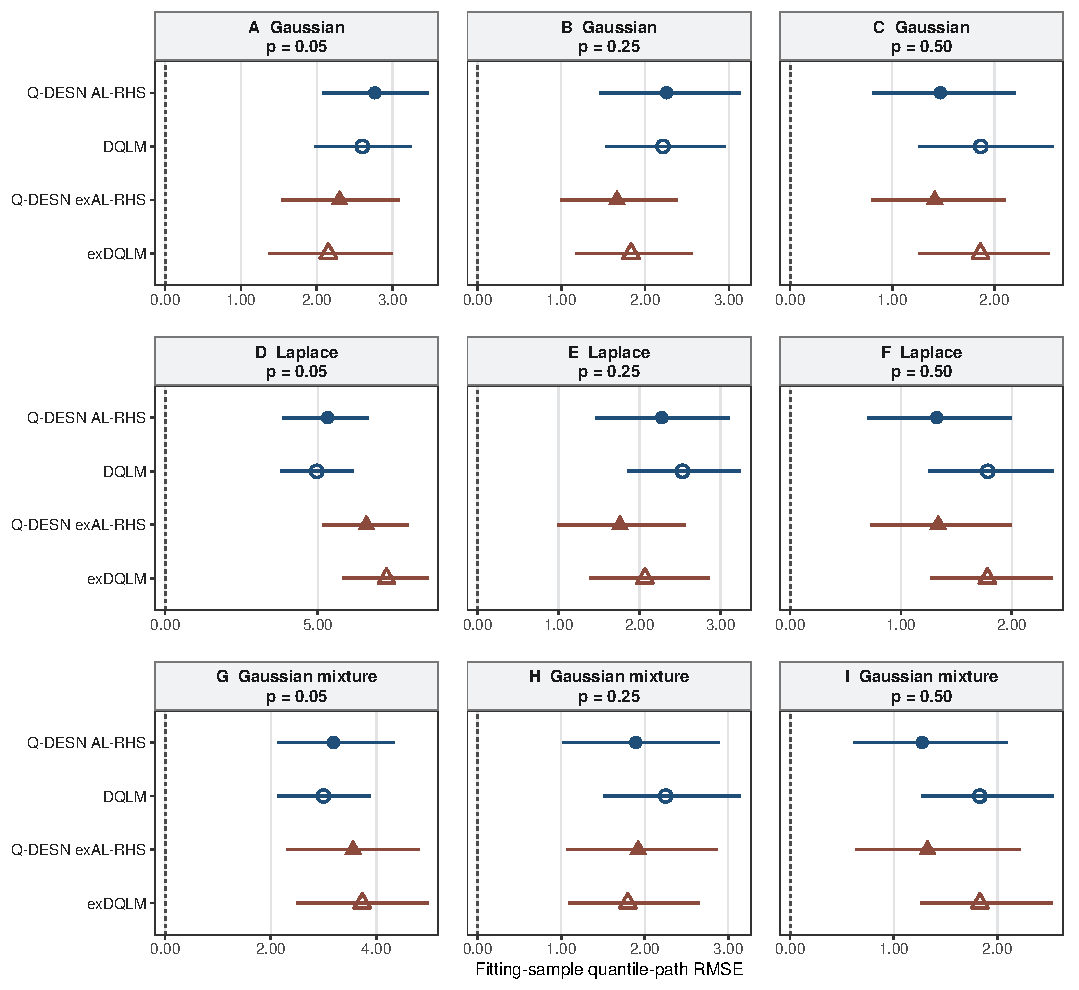
\includegraphics[width=0.98\textwidth]{figures/independent_simulation/qdesn_validation_500obs_v14_mcmc_fit_rmse_intervals.pdf}
\caption{MCMC posterior uncertainty for fitting-sample RMSE in the
single-quantile simulation. Horizontal segments show equal-tailed 95\%
posterior intervals and crosses show posterior means. Each panel has its own
horizontal scale; lower is better. The dashed line marks exact recovery of the
known conditional quantile path. Intervals condition on the simulated series
and case-specific selected specification.}
\label{fig:simulation-500obs-mcmc-fit-rmse-intervals}
\end{figure}


\begin{figure}[!htbp]
\centering
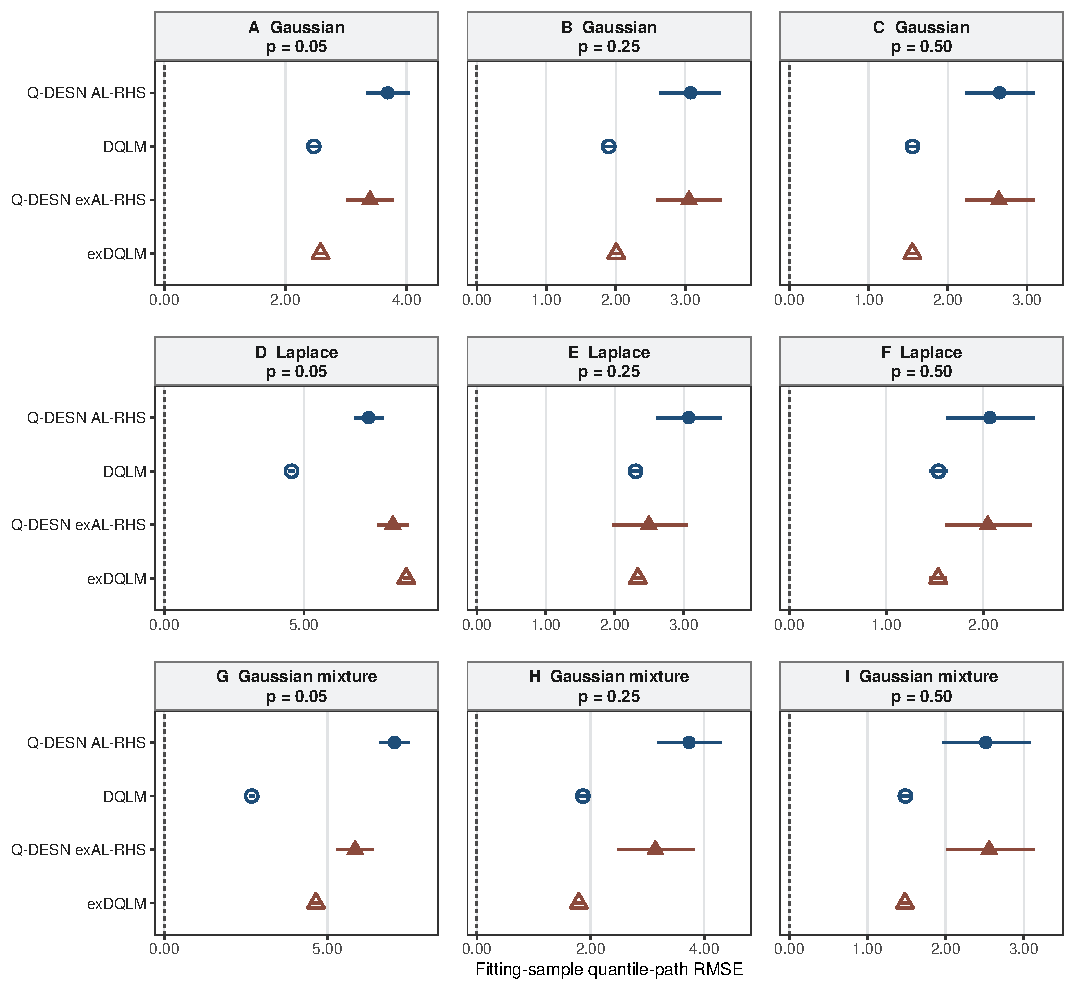
\includegraphics[width=0.98\textwidth]{figures/independent_simulation/qdesn_validation_500obs_v14_vb_fit_rmse_intervals.pdf}
\caption{Variational Bayes posterior uncertainty for fit RMSE in the single-quantile simulation study. Horizontal segments show equal-tailed approximate 95\% variational posterior intervals; crosses mark posterior means. Each panel uses its own horizontal scale, and lower values are better. The black dashed line marks the exact DGP oracle value of zero for this conditional-quantile path-error criterion. Intervals condition on the simulated data, evaluation design, and case-specific model specification.}
\label{fig:simulation-500obs-vb-fit-rmse-intervals}
\end{figure}

\begin{figure}[!htbp]
\centering
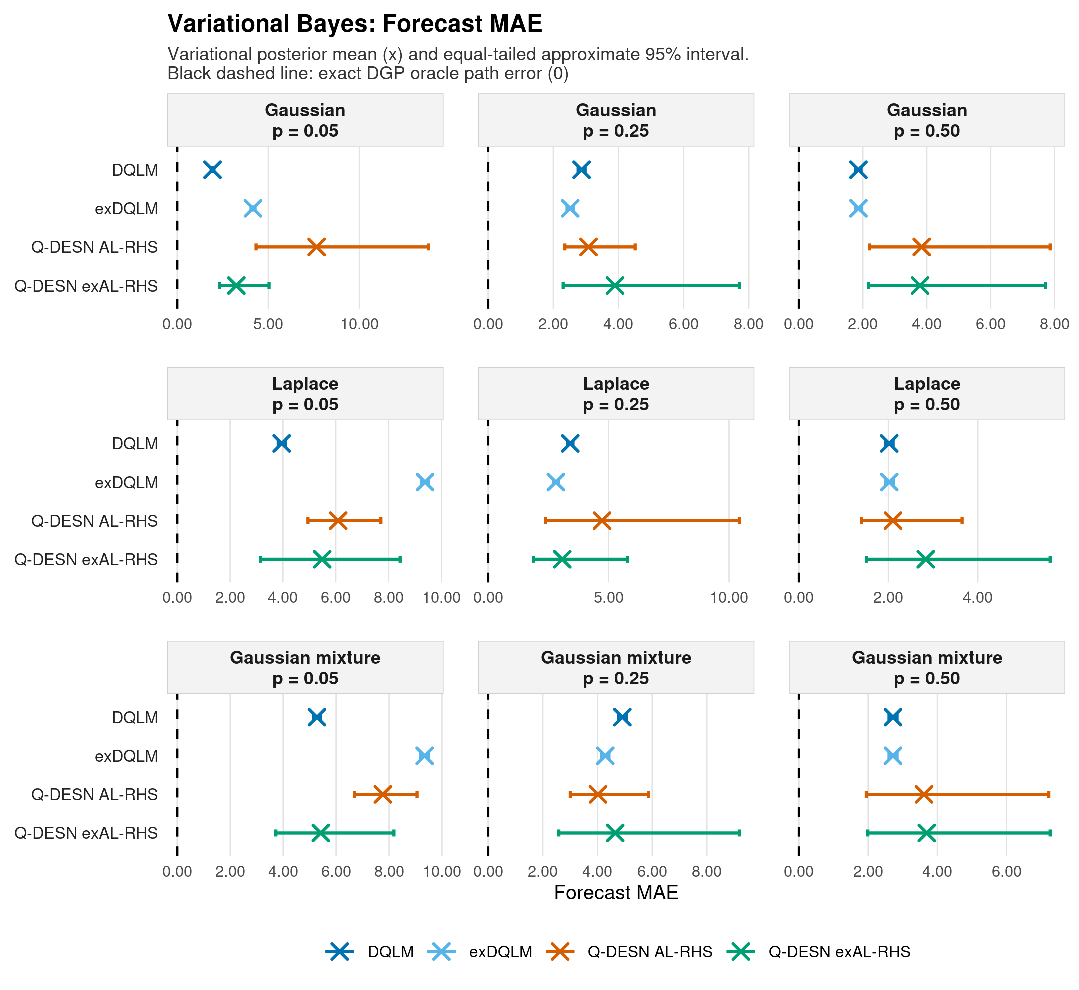
\includegraphics[width=0.98\textwidth]{figures/independent_simulation/qdesn_validation_500obs_v14_vb_forecast_mae_intervals.pdf}
\caption{Variational Bayes posterior uncertainty for forecast MAE in the single-quantile simulation study. Horizontal segments show equal-tailed approximate 95\% variational posterior intervals; crosses mark posterior means. Each panel uses its own horizontal scale, and lower values are better. The black dashed line marks the exact DGP oracle value of zero for this conditional-quantile path-error criterion. Intervals condition on the simulated data, evaluation design, and case-specific model specification.}
\label{fig:simulation-500obs-vb-forecast-mae-intervals}
\end{figure}

\begin{figure}[!htbp]
\centering
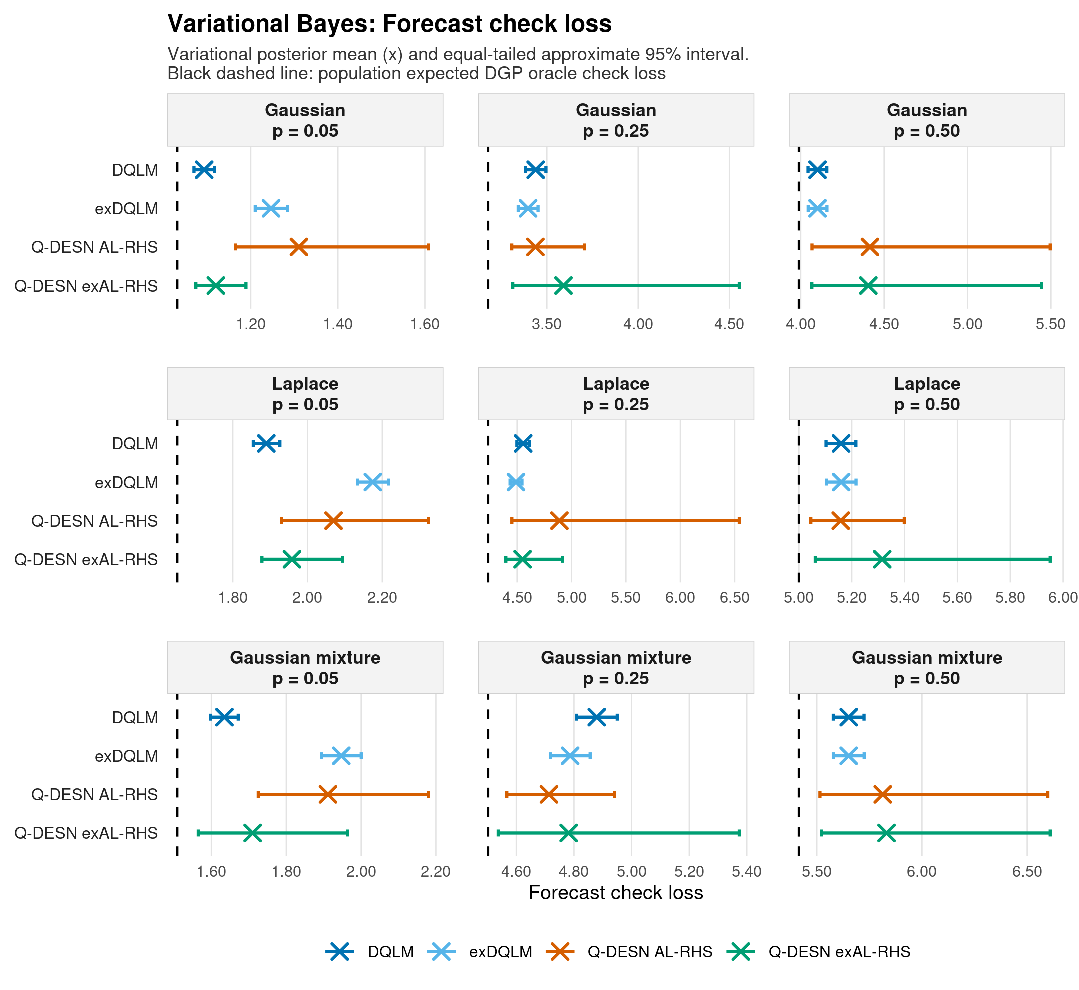
\includegraphics[width=0.98\textwidth]{figures/independent_simulation/qdesn_validation_500obs_v14_vb_forecast_check_loss_intervals.pdf}
\caption{Variational Bayes posterior uncertainty for forecast check loss in the single-quantile simulation study. Horizontal segments show equal-tailed approximate 95\% variational posterior intervals; crosses mark posterior means. Each panel uses its own horizontal scale, and lower values are better. The black dashed line marks the population expected check loss at the true conditional quantile. Because the intervals condition on one simulated series, finite-sample check-loss summaries may cross this population reference. Intervals condition on the simulated data, evaluation design, and case-specific model specification.}
\label{fig:simulation-500obs-vb-forecast-check-loss-intervals}
\end{figure}


\clearpage
\subsection{Single-Quantile Computation and Diagnostics}
\label{subsec:supp-independent-exal-mcmc-details}

The independent Q--DESN exAL--RHS MCMC analysis uses the mixture representation
for \(v\) described earlier in the supplement and an analysis-specific
scale-collapsed transition. Conditional on the remaining unknowns, the scale is
integrated from the conditional density used to update the asymmetry parameter
on a logit transformation of its bounded support, and the scale is then drawn
from its full conditional distribution. This transition is used for the
independent simulation analysis; Algorithm~\ref{alg:qdesn_mcmc} gives the generic joint or
conditionally split update. The resulting draws determine the fitted and
forecast quantile paths used in the reported criteria.

The exDQLM baseline uses version 1.1.1 of the CRAN package \pkg{exdqlm}
\citep{exdqlmRPackage}. For unrestricted exAL
fits, its MCMC sampler updates the asymmetry parameter from its conditional
distribution with the scale analytically integrated out, then draws the scale
from its full conditional distribution. Its variational calculation uses the
structured factorization \(q(\gamma)q(\sigma\mid\gamma)\). These model-specific
computations produce the
quantile-path draws evaluated by the common criteria above.
For retained pairs \((\sigma_b,\gamma_b)\),
\(b=1,\ldots,B_{\mathrm{post}}\), let
\[
m_{\varepsilon,b}=\sigma_b\{A_p(\gamma_b)+D_p(\gamma_b)\sqrt{2/\pi}\},\qquad
V_{\varepsilon,b}=\sigma_b^2\{B_p(\gamma_b)+A_p(\gamma_b)^2
  +D_p(\gamma_b)^2(1-2/\pi)\}.
\]
The rolling-origin filter uses
\(\bar m_\varepsilon=B_{\mathrm{post}}^{-1}\sum_b m_{\varepsilon,b}\) and
\(\bar V_\varepsilon=B_{\mathrm{post}}^{-1}
\sum_b(V_{\varepsilon,b}+m_{\varepsilon,b}^2)-\bar m_\varepsilon^2\).
The parameter posterior from the initial fit is retained, while observations
available at successive origins update the state filter before forecasts are
propagated over the requested horizons.

The MCMC metric distributions generally pool 12,000 retained evaluations from
three independently initialized chains. The Q--DESN AL--RHS Gaussian
\(p=0.05\) forecast MAE and check-loss summaries use 3,000 retained evaluations
from three chains. Diagnostics assess between-chain agreement for each
draw-wise criterion.

\clearpage
\subsection{Single-Quantile Five-Chain Point-Path Sensitivity}
\label{subsec:supp-independent-five-chain-sensitivity}

The primary single-quantile MCMC tables report draw-wise posterior summaries of
the evaluation criteria. The analysis below instead evaluates each criterion
on a posterior point estimate of the quantile path and provides a separate
sensitivity analysis across independently initialized chains.
For the Gaussian \(p=0.25\) comparison, a five-chain sensitivity analysis uses
five independently seeded chains for each model specification. For each chain,
the posterior point path is computed first; the reported sensitivity path is the
coordinatewise median of those five paths. All criteria are then recomputed
from that path. This construction summarizes chain-specific point estimates.

One common specification is reported for each working likelihood. Relative to
the corresponding criterion-specific summary, the \(\AL\)--\(\RHS\)
specification reduced fit RMSE by 8.4\% and forecast MAE by 1.6\%, while its
forecast check loss increased by 0.4\%. The \(\exAL\)--\(\RHS\) specification
reduced fit RMSE by 18.3\%, forecast MAE by 8.7\%, and forecast check loss by
0.4\%. Within the Gaussian \(p=0.25\) comparison, these results indicate
limited sensitivity to MCMC initialization for the selected specifications.

\begin{table}[!htbp]
\centering
\small
\setlength{\tabcolsep}{5pt}
\begin{tabular}{@{}llrrr@{}}
\toprule
Model & Comparison summary & Fit RMSE & Forecast MAE & Forecast check loss \\
\midrule
Q--DESN \(\AL\)--\(\RHS\)
  & Primary metric-specific summary & 2.176 & 2.361 & \textbf{3.297} \\
  & Five-chain coherent design & \textbf{1.993} & \textbf{2.323} & 3.309 \\
\addlinespace
Q--DESN \(\exAL\)--\(\RHS\)
  & Primary metric-specific summary & 1.710 & 2.709 & 3.333 \\
  & Five-chain coherent design & \textbf{1.396} & \textbf{2.473} & \textbf{3.319} \\
\bottomrule
\end{tabular}
\caption{Five-chain MCMC robustness sensitivity for the Gaussian simulation
family at \(p=0.25\) with 500 fitting observations. The primary rows reproduce
the metric-specific summaries in the main article's Gaussian MCMC table;
their three entries are interpreted criterion by criterion. Each five-chain
row instead uses one fixed coherent design and reports metrics recomputed from
the coordinatewise median of five chain-specific posterior point paths. This
aggregation summarizes posterior point paths across independent chains.
Forecast criteria use the held-out window of length 1000 with leads 1--30 and origin stride 30. Boldface
marks the lower value within each model and criterion. The sensitivity is
reported separately because its estimator differs from the primary table.}
\label{tab:supp-independent-mcmc-five-chain-sensitivity}
\end{table}


\clearpage
\subsection{Joint Multi-Quantile MCMC Evaluation Details}

The shared-backbone evaluation uses the initialization sequence in
Figure~\ref{fig:supp-quantile-sequential-initialization}. One scenario-specific
DESN/RHS specification is selected from source realizations and held common
across the four model classes. The evaluation realization is used only for the final
fit and evaluation. Table~\ref{tab:joint-qdesn-shared-backbone-protocol}
records the 136 variational components, 160 MCMC chains, and retained-draw
allocation.

\begin{table}[!htbp]
\centering
\scriptsize
\resizebox{\textwidth}{!}{%
\begin{tabular}{@{}>{\raggedright\arraybackslash}p{0.23\textwidth}rrrr@{}}
\toprule
Simulation setting & \shortstack{Joint Q--DESN\\\(\AL\)--\(\RHS\)} & \shortstack{Independent Q--DESN\\\(\AL\)--\(\RHS\)} & \shortstack{Joint exQDESN\\\(\exAL\)--\(\RHS\)} & \shortstack{Independent exQDESN\\\(\exAL\)--\(\RHS\)} \\
\midrule
Asymmetric-Laplace tail & 1.4617 [0.6640, 2.3337] & 0.4327 [0.3365, 0.6596] & 0.7787 [0.3639, 1.4669] & \textbf{0.3339 [0.3213, 0.3577]} \\
Gaussian-mixture innovations & 0.7138 [0.4813, 1.0255] & 0.4010 [0.3922, 0.4154] & 0.4517 [0.3922, 0.6110] & \textbf{0.3949 [0.3878, 0.4072]} \\
Laplace innovations & 0.4016 [0.3577, 0.4642] & 0.3546 [0.3351, 0.3862] & \textbf{0.3350 [0.3255, 0.3557]} & 0.3362 [0.3265, 0.3543] \\
Nonlinear reservoir dynamics & 0.4789 [0.4490, 0.5284] & 0.4332 [0.4280, 0.4403] & 0.4520 [0.4337, 0.4876] & \textbf{0.4309 [0.4259, 0.4382]} \\
Gaussian innovations & 0.3635 [0.3275, 0.4202] & 0.3576 [0.3262, 0.4046] & 0.3475 [0.3135, 0.4188] & \textbf{0.3362 [0.3161, 0.3706]} \\
Persistent heavy tails & 0.3993 [0.3660, 0.5028] & 0.3765 [0.3657, 0.3989] & 0.3891 [0.3657, 0.4454] & \textbf{0.3728 [0.3630, 0.3951]} \\
Regime shift & 0.4435 [0.4269, 0.4785] & 0.4404 [0.4277, 0.4670] & 0.4452 [0.4279, 0.4767] & \textbf{0.4373 [0.4271, 0.4617]} \\
Student-\(t\) location--scale & 0.4223 [0.3450, 0.6838] & 0.3665 [0.3481, 0.3981] & 0.3744 [0.3413, 0.4869] & \textbf{0.3545 [0.3423, 0.3805]} \\
\bottomrule
\end{tabular}
}%
\caption{Posterior data-generating-process-integrated finite-grid quantile scores for the shared-backbone joint simulation. Entries are posterior means with equal-tailed 95\% intervals from the complete shared-backbone evaluation. All four models use the same selected feature design within a simulation setting. Lower values are better; boldface marks the numerical minimum within a setting. The winner and runner-up marginal intervals overlap in every setting, so the rankings are descriptive.}
\label{tab:joint-qdesn-shared-backbone-score}
\end{table}


Figure~\ref{fig:joint-qdesn-shared-backbone-fit-rmse} compares
fitting-sample recovery under the same shared feature design used for the
forecast-score comparison in the main article.

\begin{figure}[!htbp]
\centering
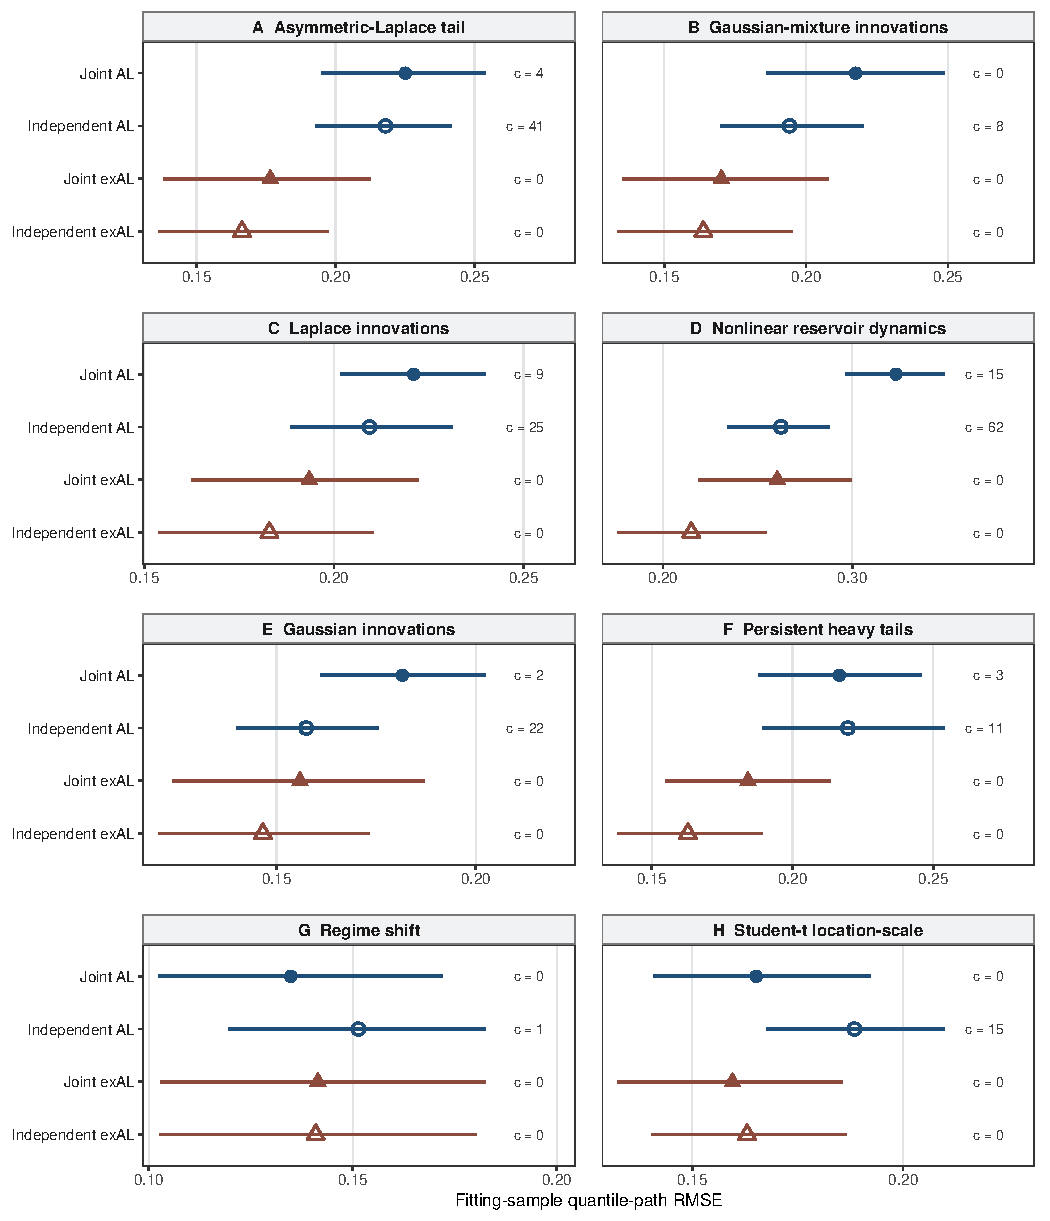
\includegraphics[width=0.94\textwidth]{figures/joint_qdesn_simulation/joint_qdesn_shared_backbone_fit_oracle_rmse_intervals.pdf}
\caption{Posterior fitting-sample recovery of the known conditional quantile
paths under the shared-backbone design. Points are posterior means of
quantile-path RMSE and horizontal segments are equal-tailed 95\% intervals
after monotone rearrangement; lower values are better. Navy circles identify
the \(\AL\) models and muted-brick triangles the \(\exAL\) models; filled
symbols denote joint fits and open symbols independent fits. Panels A--H
identify the data-generating mechanism and use separate horizontal scales.
Labels \(c\) give raw crossings in the posterior-mean grid; all counts after
rearrangement are zero.}
\figalt{Eight panels compare posterior fitting-sample quantile-path RMSE means
and 95 percent intervals for joint and independent AL and exAL models. Each
model is annotated with its number of raw quantile crossings; all rearranged
grids have zero crossings.}
\label{fig:joint-qdesn-shared-backbone-fit-rmse}
\end{figure}


The posterior-score diagnostics satisfy the pre-specified rank-normalized
\(\widehat R\), effective-sample-size, and Monte Carlo error criteria in 21 of
32 comparisons; the other 11 are retained with review status. All 16
\(\exAL\) scale--asymmetry assessments are also retained at review level.
Precision stabilization was enabled for 96 \(\exAL\) chains and invoked in
eight chains for 34 coefficient updates; the maximum relative diagonal
perturbation was \(10^{-12}\). All repaired chains satisfy the numerical
checks and no result is excluded on this basis.

Five paired joint-minus-independent score intervals lie entirely above zero,
favoring independent estimation, and the other eleven include zero. Raw
crossings are reported separately from the score after monotone
rearrangement. All
posterior-mean grids are ordered after rearrangement.

\begin{table}[!htbp]
\centering
\small
\begin{tabular}{@{}>{\raggedright\arraybackslash}p{0.25\textwidth}>{\raggedright\arraybackslash}p{0.65\textwidth}@{}}
\toprule
Item & Value \\
\midrule
Feature design & One scenario-specific DESN/RHS specification selected from independent source realizations and then shared by all four model classes; the evaluation realization was not used for selection. \\
Quantile grid & 0.05, 0.10, 0.25, 0.50, 0.75, 0.90, and 0.95. \\
Sequential initialization & Gaussian ridge to Gaussian RHS--VB; then median-centered independent AL continuation, matching AL-to-exAL initialization, complete independent grids to the corresponding joint fit, and matching VB-to-MCMC initialization. \\
VB calculation & 136 components: 8 Gaussian RHS, 56 independent AL, 56 independent exAL, 8 joint AL, and 8 joint exAL fits. \\
MCMC calculation & 160 independently seeded chains. Each AL cell uses four chains of 4,000 iterations with 1,000 burn-in and thinning by 4; each exAL cell uses six chains of 8,000 iterations with 2,000 burn-in and thinning by 4. \\
Posterior score summary & 3,000 chain-balanced draws per AL cell and 4,500 per exAL cell; entries are posterior means with equal-tailed 95\% intervals. \\
Forecast evaluation & 990 aligned, sequentially conditional origin--horizon rows per comparison. The DGP-integrated seven-level score is computed after monotone rearrangement. \\
\bottomrule
\end{tabular}
\caption{Design of the shared-backbone joint multi-quantile evaluation. Initialization transfers starting values only; each destination retains its own likelihood, prior, and posterior target.}
\label{tab:joint-qdesn-shared-backbone-protocol}
\end{table}

\begin{table}[!htbp]
\centering
\small
\begin{tabular}{@{}>{\raggedright\arraybackslash}p{0.39\textwidth}rr@{}}
\toprule
Simulation setting & \(\AL\) & \(\exAL\) \\
\midrule
Asymmetric-Laplace tail & \textbf{1.0290 [0.2019, 1.9156]} & \textbf{0.4448 [0.0299, 1.1317]} \\
Gaussian-mixture innovations & \textbf{0.3128 [0.0789, 0.6241]} & 0.0568 [-0.0052, 0.2175] \\
Laplace innovations & 0.0470 [-0.0060, 0.1125] & -0.0012 [-0.0225, 0.0220] \\
Nonlinear reservoir dynamics & \textbf{0.0456 [0.0152, 0.0958]} & \textbf{0.0211 [0.0009, 0.0573]} \\
Gaussian innovations & 0.0060 [-0.0534, 0.0714] & 0.0112 [-0.0392, 0.0835] \\
Persistent heavy tails & 0.0228 [-0.0202, 0.1256] & 0.0163 [-0.0162, 0.0730] \\
Regime shift & 0.0032 [-0.0301, 0.0421] & 0.0079 [-0.0234, 0.0423] \\
Student-\(t\) location--scale & 0.0559 [-0.0343, 0.3230] & 0.0199 [-0.0267, 0.1297] \\
\bottomrule
\end{tabular}
\caption{Joint-minus-independent posterior contrasts in the DGP-integrated finite-grid quantile score. Entries are means with equal-tailed 95\% intervals under the pre-specified chain-balanced pairing. Positive values favor independent estimation. Boldface marks the five intervals lying entirely above zero; the other eleven include zero.}
\label{tab:supp-joint-qdesn-shared-backbone-contrasts}
\end{table}

\begin{table}[!htbp]
\centering
\small
\begin{tabular}{@{}>{\raggedright\arraybackslash}p{0.42\textwidth}rrrr@{}}
\toprule
Model & \shortstack{Fit\\raw} & \shortstack{Forecast\\raw} & \shortstack{After\\rearrangement} & \shortstack{Mean forecast draw\\crossing rate (\%)} \\
\midrule
Joint Q--DESN \(\AL\)--\(\RHS\) & 33 & 1426 & 0 & 6.21 \\
Independent Q--DESN \(\AL\)--\(\RHS\) & 185 & 4705 & 0 & 15.17 \\
Joint exQDESN \(\exAL\)--\(\RHS\) & 0 & 0 & 0 & 1.60 \\
Independent exQDESN \(\exAL\)--\(\RHS\) & 0 & 281 & 0 & 11.20 \\
\bottomrule
\end{tabular}
\caption{Adjacent-level crossings for posterior-mean quantile grids, summed over the eight simulation settings. Raw counts are reported before monotone rearrangement; all 32 grids are ordered afterward. The final column averages the draw-level forecast crossing rate across settings.}
\label{tab:supp-joint-qdesn-shared-backbone-crossings}
\end{table}

\begin{table}[!htbp]
\centering
\scriptsize
\resizebox{\textwidth}{!}{%
\begin{tabular}{@{}>{\raggedright\arraybackslash}p{0.23\textwidth}rrrr@{}}
\toprule
Simulation setting & \shortstack{Joint Q--DESN\\\(\AL\)--\(\RHS\)} & \shortstack{Independent Q--DESN\\\(\AL\)--\(\RHS\)} & \shortstack{Joint exQDESN\\\(\exAL\)--\(\RHS\)} & \shortstack{Independent exQDESN\\\(\exAL\)--\(\RHS\)} \\
\midrule
Asymmetric-Laplace tail & 1.639 (2.160) & 0.414 (0.656) & 0.858 (1.091) & 0.143 (0.236) \\
Gaussian-mixture innovations & 0.808 (1.041) & 0.205 (0.286) & 0.280 (0.367) & 0.097 (0.122) \\
Laplace innovations & 0.330 (0.477) & 0.265 (0.378) & 0.147 (0.186) & 0.141 (0.181) \\
Nonlinear reservoir dynamics & 0.418 (0.582) & 0.211 (0.317) & 0.243 (0.300) & 0.134 (0.172) \\
Gaussian innovations & 0.307 (0.390) & 0.281 (0.334) & 0.239 (0.287) & 0.202 (0.249) \\
Persistent heavy tails & 0.251 (0.304) & 0.192 (0.264) & 0.152 (0.194) & 0.096 (0.120) \\
Regime shift & 0.178 (0.200) & 0.131 (0.156) & 0.210 (0.251) & 0.125 (0.148) \\
Student-\(t\) location--scale & 0.310 (0.385) & 0.416 (0.671) & 0.184 (0.226) & 0.089 (0.116) \\
\bottomrule
\end{tabular}
}%
\caption{Forecast recovery of the known conditional quantile paths. Entries are mean absolute error with root-mean-square error in parentheses for the monotonically rearranged posterior-mean forecast grids. All four models use the same selected feature design within each setting.}
\label{tab:supp-joint-qdesn-shared-backbone-oracle}
\end{table}

\begin{table}[!htbp]
\centering
\scriptsize
\begin{tabular}{@{}>{\raggedright\arraybackslash}p{0.30\textwidth}rrr@{}}
\toprule
Scenario & Joint: AL-exAL & Independent: AL-exAL & Replicates
\\
\midrule
Asymmetric Laplace Tail & -0.054 (100\%) & -0.042 (94\%) & 50 \\
Gaussian-Mixture Bridge & -0.047 (96\%) & -0.045 (96\%) & 50 \\
Laplace Bridge & -0.045 (96\%) & -0.037 (92\%) & 50 \\
Nonlinear Reservoir Friendly & -0.047 (94\%) & -0.044 (94\%) & 50 \\
Normal Bridge & -0.031 (94\%) & -0.027 (92\%) & 50 \\
Persistent Heavy Tail & -0.035 (88\%) & -0.031 (82\%) & 50 \\
Regime Shift & -0.037 (70\%) & -0.041 (96\%) & 50 \\
Student-t Location-Scale & -0.043 (86\%) & -0.037 (84\%) & 50 \\
\bottomrule
\end{tabular}
\caption{Replicated VB comparison of AL and exAL forecast quantile-path MAE over 50 independent data-generating realizations per scenario. Entries are the median paired difference AL minus exAL, with the percentage of replicates favoring AL in parentheses.}
\label{tab:joint-qdesn-article-validation-phase153-replication-summary}
\end{table}



The displayed shared-backbone calculations used the RHS global-scale update present in
the stored calculation. If \(d_\beta\) denotes the number of penalized
coefficients in a global-scale block, a subsequent source correction changed
the shape term in that conditional update from \(d_\beta/2\) to
\((d_\beta+1)/2\). No numerical
adjustment has been made to the stored results. A confirmatory rerun under the
corrected update is registered as required before the final archival release;
until then, this complete shared-backbone analysis is the provisional article
authority.

The final table reports a separate 50-replicate variational sensitivity
analysis. Its paired \(\AL\)-minus-\(\exAL\) forecast-MAE differences assess
recovery of the known quantile paths; the MCMC DGP-integrated score remains
the ranking criterion in the main comparison.

\clearpage
\subsection{Additional PriceFM Results}
\label{subsec:supp_pricefm_diagnostics}

The main article reports the aggregate, fold-specific, and forecast-lead-specific
PriceFM comparisons. The tables below compare the selected and reference
Q--DESN specifications and summarize results by predictor set. Both use the
retrospective information set described in the main article.

Within \PricefmSelectionComparedRows{} region--fold comparisons, AL and exAL
specifications were chosen using validation AQL and then evaluated on held-out
observations. The validation-selected specifications averaged test AQL
\PricefmSelectionCandidateMeanAql{}, compared with
\PricefmSelectionReferenceMeanAql{} for the reference Q--DESN specifications.
The reported aggregate uses the validation-selected specification in the
\PricefmSelectionUpdatedRows{} cases listed in
Table~\ref{tab:supp-pricefm-selective-updates}, where its held-out AQL was lower
than both the reference Q--DESN and matched PriceFM values.
The retained alternatives use exAL except for ES fold~1, which uses AL. Only
IT\_NORD fold~3 changes the working-likelihood family relative to the reference
specification. The comparisons are descriptive because held-out performance
determined which specification was included.

\begin{table}[!htbp]
\centering
\caption{Comparison of selected and reference Q--DESN specifications in the
PriceFM retrospective analysis. Each row gives a validation-selected
specification whose held-out AQL is lower than both the reference Q--DESN value
and the matched PriceFM value. The final column is the reduction from the
reference Q--DESN AQL. Values are reported on the original electricity-price
scale.}
\label{tab:supp-pricefm-selective-updates}
\resizebox{\textwidth}{!}{%
\begingroup
\TableStyle
\scriptsize
\setlength{\tabcolsep}{4pt}
\begin{tabular}{@{}llrrrr@{}}
\toprule
Region--fold & Working likelihood & Updated Q--DESN AQL & Reference Q--DESN AQL & PriceFM AQL & AQL reduction \\
\midrule
IT\_NORD--3 & \(\exAL\) & 4.455446 & 4.584470 & 5.840089 & 0.129024 \\
SE\_3--1 & \(\exAL\) & 7.563096 & 7.620994 & 7.628088 & 0.057899 \\
IT\_CNOR--1 & \(\exAL\) & 4.692527 & 4.723481 & 5.940016 & 0.030955 \\
DK\_2--2 & \(\exAL\) & 6.314902 & 6.331814 & 8.251471 & 0.016913 \\
HU--1 & \(\exAL\) & 7.871386 & 7.884141 & 8.500270 & 0.012755 \\
ES--1 & \(\AL\) & 5.232137 & 5.243147 & 5.959308 & 0.011010 \\
DK\_2--3 & \(\exAL\) & 7.407690 & 7.411013 & 9.368512 & 0.003323 \\
AT--1 & \(\exAL\) & 6.739250 & 6.741377 & 7.402188 & 0.002127 \\
LV--3 & \(\exAL\) & 12.838358 & 12.840327 & 13.756953 & 0.001969 \\
FR--3 & \(\exAL\) & 5.719495 & 5.720239 & 6.817623 & 0.000743 \\
BE--2 & \(\exAL\) & 6.396754 & 6.396922 & 6.496657 & 0.000167 \\
DK\_1--3 & \(\exAL\) & 7.212994 & 7.213099 & 7.943293 & 0.000105 \\
\bottomrule
\end{tabular}
\endgroup

}
\end{table}

\begin{table}[!htbp]
\centering
\caption{PriceFM retrospective comparison by predictor set. Own-region rows and rows with
neighborhood summaries both use retrospectively observed own-region load,
solar, and wind lead covariates in the retrospective comparison. Rows with
neighborhood summaries additionally include chosen neighboring-region
summaries or neighboring-region lead/lag features. The two PriceFM columns
count relative AQL advantages of at most 5\% and greater than 5\%, respectively.}
\label{tab:supp-pricefm-full-input-set-summary}
\begingroup
\TableStyle
\scriptsize
\setlength{\tabcolsep}{3pt}
\begin{tabular}{@{}lrrrrrr@{}}
\toprule
Input set & $n$ & \shortstack{Q--DESN\\lower} & \shortstack{Near\\ties} & \shortstack{PriceFM\\lower} & \shortstack{Mean\\$\Delta$} & \shortstack{Median\\$\Delta$} \\
\midrule
Neighboring-region predictors & 56 & 34 & 5 & 17 & -0.368 & -0.113 \\
Own-region predictors & 58 & 32 & 7 & 19 & -0.068 & -0.056 \\
\bottomrule
\end{tabular}
\endgroup

\end{table}

\clearpage
\section{GloFAS Latent-Path Ensemble-Likelihood Model with DESN Features}
\label{sec:glofas_discrepancy}

\noindent\textbf{Model overview.}
The streamflow application combines the historical and issued Global Flood
Awareness System (GloFAS) products with a reference gauge record
\citep{AlfieriEtAl2013GloFAS,HarriganEtAl2023GloFASForecasts}. Separate DESN
feature maps represent the reference process and the GloFAS-minus-reference
discrepancy. The selected Part 4 analysis is a joint AL--RHS variational fit:
post-cutoff reference values are latent during fitting, and the issued ensemble
contributes directly to the same latent-path analysis. It is not a post-fit
forecast adjustment.

\subsection{Observed Quantities and Latent Design}
\label{subsec:glofas_aug_design}

Let \(T\) denote 25~December~2022 and let
\(y_t=\log(y_t^{\mathrm{USGS}}+1)\) be transformed reference streamflow.
Write \(g_t^{\mathrm{ret}}\) for transformed retrospective GloFAS and
\(g_{T+h,e}^{\mathrm{ens}}\) for transformed issued member \(e\) at horizon
\(h\). The requested future path
\(\vect y_F=(y_{T+1},\ldots,y_{T+30})^\top\) is unobserved during fitting.
Issued GloFAS values are available for the first 28 horizons, with 51 members
at each horizon. The withheld USGS values are loaded only after fitting for
forecast evaluation. Realized PRISM/ERA5 precipitation and soil-moisture
covariates are used after \(T\), so the calculation is a retrospective
oracle-covariate diagnostic.

For probability level \(p_k\), the reference and discrepancy quantile
locations are
\begin{equation}
\begin{aligned}
\text{Reference quantile:}\quad
q_{k,t}
&=\vect x_t^{\mathrm{ref}\top}\vect\beta_k,\\
\text{Discrepancy quantile:}\quad
d_{k,t}
&=\vect x_t^{\mathrm{disc}\top}\vect\delta_k,\\
\text{GloFAS quantile:}\quad
q_{k,t}^{\mathrm{glo}}
&=q_{k,t}+d_{k,t}.
\end{aligned}
\label{eq:supp_glofas_quantile_decomposition}
\end{equation}
Historical reference features are generated from the observed reference
history, and historical discrepancy features are generated from
\(g_t^{\mathrm{ret}}-y_t\). After \(T\), the reference and discrepancy
reservoir states are recomputed as functions of the latent path
\(\vect y_F\). Strict lagging is imposed: the design row for \(T+h\) may
depend on earlier latent values but not on \(y_{T+h}\).

For one probability level, stack the reference and discrepancy coefficients as
\[
\vect\theta_k=
\begin{bmatrix}\vect\beta_k\\ \vect\delta_k\end{bmatrix},
\qquad
\vect h_t^{\mathrm{ref}}=
\begin{bmatrix}\vect x_t^{\mathrm{ref}}\\ \vect 0\end{bmatrix},
\qquad
\vect h_t^{\mathrm{glo}}=
\begin{bmatrix}\vect x_t^{\mathrm{ref}}\\
\vect x_t^{\mathrm{disc}}\end{bmatrix}.
\]
Then \(\vect h_t^{\mathrm{ref}\top}\vect\theta_k=q_{k,t}\) and
\(\vect h_t^{\mathrm{glo}\top}\vect\theta_k=q_{k,t}+d_{k,t}\).
Conditional on \(\vect y_F\), these are ordinary fixed-design Q--DESN
regressions.

The selected reference reservoir has depth one, width
\(\GlofasApplicationCurrentReferenceReservoirSize{}\), memory
\(\GlofasApplicationCurrentReferenceReservoirMemory{}\), leak rate
\(\GlofasApplicationCurrentReferenceReservoirAlpha{}\), spectral radius
\(\GlofasApplicationCurrentReferenceReservoirRho{}\), washout
\(\GlofasApplicationCurrentReferenceReservoirWashout{}\), and seed
\(\GlofasApplicationCurrentReferenceReservoirSeed{}\). Its inputs are reference
lags 1--360 and realized precipitation and soil-moisture lags 0--180. The
discrepancy reservoir has width
\(\GlofasApplicationCurrentDiscrepancyReservoirSize{}\), memory
\(\GlofasApplicationCurrentDiscrepancyReservoirMemory{}\), leak rate
\(\GlofasApplicationCurrentDiscrepancyReservoirAlpha{}\), spectral radius
\(\GlofasApplicationCurrentDiscrepancyReservoirRho{}\), washout
\(\GlofasApplicationCurrentDiscrepancyReservoirWashout{}\), and seed
\(\GlofasApplicationCurrentDiscrepancyReservoirSeed{}\). It uses the
corresponding discrepancy and weather lags. Neither feature map includes
direct readout inputs. The reference and discrepancy RHS scales are
\(\tau_{0,\mathrm{ref}}=\GlofasApplicationCurrentSharedRhsTau{}\) and
\(\tau_{0,\mathrm{disc}}=\GlofasApplicationCurrentDiscrepancyRhsTau{}\).

\subsection{Weighted Augmented Working Likelihood}
\label{subsec:glofas_likelihoods}

At each level \(p_k\), reference observations have AL location \(q_{k,t}\),
whereas retrospective and issued GloFAS observations have location
\(q_{k,t}+d_{k,t}\). Let \(z_i^c\) and \(\vect h_i^c\) denote an observation
and design row from source \(c\in\{\mathrm{ref},\mathrm{glo}\}\). The AL
normal--exponential augmentation is
\begin{equation}
\begin{aligned}
\text{Latent scale:}\quad
v_{i,k}^c\mid\sigma_{c,k}
&\sim\Exp(\mathrm{rate}=1/\sigma_{c,k}),\\
\text{Conditional observation:}\quad
z_i^c\mid\cdot
&\sim\Normal\!\left(
\vect h_i^{c\top}\vect\theta_k+A_{0,k}v_{i,k}^c,\,
\sigma_{c,k}B_{0,k}v_{i,k}^c
\right).
\end{aligned}
\label{eq:supp_glofas_al_hierarchy}
\end{equation}

Define an observation weight \(w_i=1\) for historical reference and
retrospective GloFAS rows. For an issued member at a fixed horizon,
\(w_i=1/51\). Hence the 51 issued members contribute total weight one at each
horizon. The executed augmented working likelihood has the form
\begin{equation}
\begin{aligned}
\text{Weighted augmented likelihood:}\quad
L_{\mathrm{aug}}(\Theta)
\ \propto\
\prod_{k=1}^{K}\prod_{c}\prod_{i\in\mathcal I_c}
\left[
p(z_i^c\mid v_{i,k}^c,\Theta_k)\,
p(v_{i,k}^c\mid\sigma_{c,k})
\right]^{w_i}.
\end{aligned}
\label{eq:supp_glofas_weighted_augmented_likelihood}
\end{equation}
This is a complete-data fractional or power-likelihood construction. It
prevents the issued ensemble from receiving 51 times the weight of one
historical time point. Because the power is applied before integrating out the
latent variables, Eq.~\eqref{eq:supp_glofas_weighted_augmented_likelihood} is
not asserted to be an exact fractional marginal AL posterior.

The source-specific scales, coefficient priors, and latent variables are
updated under this weighted augmentation. The exAL comparator additionally
contains source-specific shape parameters and positive-shift latent variables,
using the structured quadrature calculations described earlier. The selected
application result uses AL, not exAL.

\subsection{Joint Quantile and Latent-Path Approximation}
\label{subsec:glofas_latent_path}

The fitted grid is
\[
(0.05,\ 0.20,\ 0.35,\ 0.50,\ 0.65,\ 0.80,\ 0.95).
\]
The seven reference coefficient blocks and seven discrepancy coefficient
blocks are linked by separate adjacent-quantile RHS priors. Computation uses
mean-field quantile-block coordinate updates initialized from the completed
independent fits. The construction shares information through these priors; it
is not a single exact Gaussian update over every coefficient and latent-path
block.

Let \(\ell_F(\vect y_F)\) be the expected weighted augmented log likelihood,
under the other current variational factors, for terms whose response or
design depends on \(\vect y_F\). At its mode
\(\widehat{\vect y}_F\), the latent-path factor is approximated by
\begin{equation}
\begin{aligned}
\text{Latent-path factor:}\quad
\mat K_F&=-\nabla^2\ell_F(\widehat{\vect y}_F),&
q_F(\vect y_F)&\approx
\Normal(\widehat{\vect y}_F,\mat K_F^{-1}).
\end{aligned}
\label{eq:supp_glofas_future_path_factor}
\end{equation}
For design row \(\vect h_i^c(\vect y_F)\), let \(\mat J_i\) be its Jacobian at
the mode and \(\mat V_F=\mat K_F^{-1}\). The first-order moments propagated to
the remaining updates are
\begin{equation}
\begin{aligned}
\text{Propagated design moments:}\quad
\E\{\vect h_i^c(\vect y_F)\}
&\approx \vect a_i^c,\\
\E\{\vect h_i^c\vect h_i^{c\top}\}
&\approx \vect a_i^c\vect a_i^{c\top}
+\mat J_i\mat V_F\mat J_i^\top,
\end{aligned}
\label{eq:supp_glofas_future_path_delta}
\end{equation}
where \(\vect a_i^c=\vect h_i^c(\widehat{\vect y}_F)\). The corresponding
Jacobian--covariance term is retained for cross-moments involving a component
of \(\vect y_F\). This gives a Laplace--Delta approximation to the nonlinear
latent-path objective. No separate forecast adapter, future-response
imputation from the withheld truth, or post-hoc crossing correction is used.

\subsection{Numerical Qualification and Supplementary Results}
\label{subsec:glofas_checks}

The inherited 50-iteration RHS warmup corresponds to five joint outer sweeps
because every sweep contains at least ten inner coefficient iterations. The
retained source fit completed those five sweeps without a global-scale update.
The continuation preserved that fitted state, released the global scales at
sweep 6, and completed five post-release updates through sweep 10. All inner
fits converged, the RHS gate passed, and every one of the 14 reference and
discrepancy RHS blocks changed after release. The final maximum parameter
change was \(0.004153866\), exceeding the strict outer tolerance \(0.001\).
Accordingly, the selected Joint AL estimate is cap-stabilized after RHS
release, not strictly outer-converged. The optional Joint exAL continuation was
stopped; its source fit is retained only as a nonconverged sensitivity result.
No MCMC fit was used for this application.

\begin{table}[!htbp]
\centering
\resizebox{\textwidth}{!}{%
\begin{tabular}{lrrrrr}
\toprule
Model & CRPS (log1p) & CRPS (original) & Coverage & CPU hours & Numerical status \\
\midrule
Normal Ridge & 0.8062 & 32.032 & 0.250 & 0.29 & completed \\
Joint AL & 0.8374 & 27.132 & 0.929 & 93.00 & cap stabilized after rhs release \\
Independent AL & 0.8606 & 28.053 & 0.929 & 8.00 & completed \\
Normal RHS/VB & 0.9412 & 33.858 & 0.179 & 0.42 & completed \\
Joint exAL & 1.0063 & 31.829 & 0.786 & 15.87 & source fit not qualified \\
Independent exAL & 1.0478 & 32.787 & 0.750 & 9.65 & completed \\
Raw GloFAS & 1.4360 & 39.401 & 0.000 & 0.00 & completed \\
\bottomrule
\end{tabular}
}
\caption{Part 4 issued-window comparison on the transformed scale. The Normal
rows are diagnostic baselines. Joint AL is the selected quantile model; its
numerical status is cap-stabilized after RHS release. Joint exAL is retained
only as a nonconverged sensitivity result. CRPS is the seven-level integrated
check-loss approximation.}
\label{tab:supp-glofas-part4-family-scores}
\end{table}

\begin{table}[!htbp]
\centering
\begin{tabular}{lrrr}
\toprule
Historical window & FR09 CRPS & Part 4 Joint AL CRPS & Relative change \\
\midrule
all & 0.0438 & 0.0739 & +68.6\% \\
last1000 & 0.0269 & 0.0549 & +104.2\% \\
last200 & 0.0389 & 0.0589 & +51.4\% \\
last50 & 0.1307 & 0.1419 & +8.6\% \\
\bottomrule
\end{tabular}

\caption{Historical CRPS guardrail on the common six-level grid. Positive
relative changes indicate larger CRPS for Part 4 Joint AL. FR09 remains the
stronger historical-fit benchmark; Part 4 authority is confined to the
single-origin issued-window experiment.}
\label{tab:supp-glofas-part4-historical-guardrail}
\end{table}

\begin{figure}[!htbp]
\centering
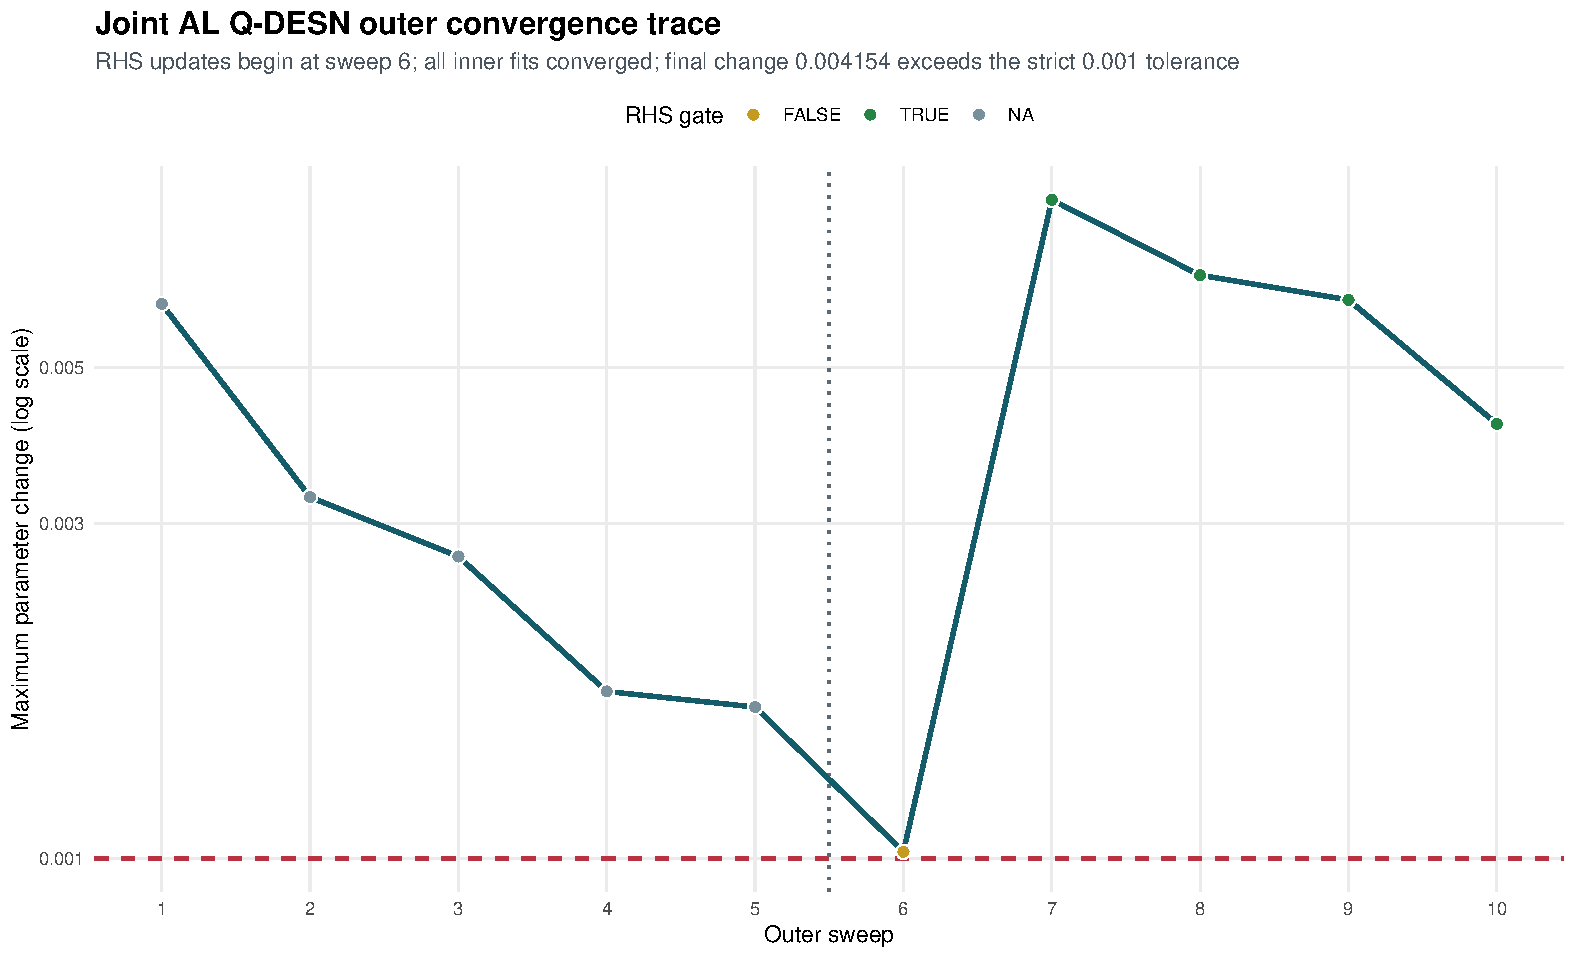
\includegraphics[width=0.94\textwidth]{figures/glofas_application/diagnostics/glofas_part4_joint_al_convergence_trace__glofas_part4_joint_al_sweep10_20260911.pdf}
\caption{Outer-iteration parameter-change trace for the selected Joint AL fit.
The vertical dotted line marks release of the RHS global scales after sweep 5,
and the horizontal dashed line marks the strict \(0.001\) outer tolerance.
The fit reached sweep 10 with all inner and RHS conditions satisfied, but the
final change remained above the strict tolerance.}
\figalt{The maximum parameter change decreases across ten outer sweeps but
remains above the strict tolerance. RHS global-scale updates begin at sweep 6.}
\label{fig:supp-glofas-part4-convergence}
\end{figure}

Removing the GloFAS source and discrepancy coefficients recovers the ordinary
Q--DESN regression. Holding the future path fixed recovers the fixed-design
updates. Strict forecast lagging, the future-truth firewall, source indexing,
horizon weights, RHS release certificate, and agreement between the stored and
reconstructed score summaries provide implementation checks. Posterior
calibration beyond this single origin remains an empirical question.

\bibliographystyle{apalike}
\bibliography{refs}

\end{document}
